\documentclass[12pt,a4paper,titlepage]{article}

\usepackage{ifplatform}  % needed to input conditionals to achieve platform-independent code

\usepackage[bitstream-charter]{mathdesign}

\usepackage[T1]{fontenc}

\usepackage{amsmath}
\usepackage{bm}

\DeclareMathOperator{\dom}{dom}
\DeclareMathOperator{\ran}{ran}
\DeclareMathOperator{\per}{period}
\DeclareMathOperator{\lcm}{lcm}
\DeclareMathOperator{\E}{E}
\DeclareMathOperator{\Var}{Var}
\DeclareMathOperator{\sd}{sd}
\DeclareMathOperator{\Bi}{Bi}
\DeclareMathOperator{\Hypergeometric}{Hypergeometric}

\newcommand{\diff}[2][]{\frac{\text{d}#1}{\text{d}#2}}
\newcommand{\intd}[1]{\text{ d}#1}

\usepackage{mathtools}

\DeclarePairedDelimiter {\pars}  {  (      }     {  )      }
\DeclarePairedDelimiter {\bracs} {  [      }     {  ]      }
\DeclarePairedDelimiter {\curls} { \{      }     { \}      }
\DeclarePairedDelimiter {\verts} { \lvert  }     { \rvert  }

\everymath{\displaystyle}  % Use \textstyle for "normal" inline math

\usepackage{siunitx}

\usepackage[dvipsnames, cmyk]{xcolor}
\selectcolormodel{natural}
\usepackage{ninecolors}
\selectcolormodel{cmyk}

\usepackage{varwidth}

\usepackage{tcolorbox}
\tcbuselibrary{skins, theorems, breakable, minted}

\usepackage{tabularray}

\usepackage{pgfplots}
\pgfplotsset{%
    compat=1.18,
    My Style 1/.style={%
        axis lines=middle,
        xlabel={$x$},
        ylabel={$y$},
        samples=150,
        xtick=\empty,
        ytick=\empty,
        label style={font=\footnotesize},
        axis equal,
        major tick style={semithick}
    },
    My Style 2/.style={%
        axis lines=middle,
        xlabel={$x$},
        ylabel={$y$},
        samples=300,
        label style={font=\footnotesize},
        ticklabel style={font=\footnotesize},
        major tick style={semithick},
        height=4.8cm,
        scale only axis,
        restrict y to domain=-2:2
    }
}

\tikzset{%
    shaded area/.style={fill=BlueGreen},
    ->-/.style={decoration={markings, mark=at position 0.2 with {\arrow{>}}}, postaction={decorate}},
    ->>-/.style={decoration={markings, mark=at position 0.2 with {\arrow{>>}}}, postaction={decorate}}
}

\pgfmathdeclarefunction{gauss}{2}{%
    \pgfmathparse{%
        1/(#2*sqrt(2*pi))*exp(-((x-#1)^2)/(2*#2^2))%
    }%
}

\usetikzlibrary{decorations.pathreplacing, decorations.markings, arrows.meta, positioning, intersections, external}
\tikzexternalize[prefix=figures/]

\usepackage{float}

\usepackage{enumitem}
\setitemize{noitemsep,topsep=0pt,parsep=4pt,partopsep=0pt,leftmargin=*}
\setlist[itemize,1]{label={\scriptsize\raisebox{0.35ex}{$\blacksquare$}}}
\setlist[itemize,2]{label=$\bullet$}

\usepackage{multicol}

\usepackage[margin=2cm]{geometry}

\usepackage{pdflscape}

\usepackage{tocloft}

%\addtolength{\cftpartnumwidth}{10pt}
\addtolength{\cftsecnumwidth}{10pt}
\addtolength{\cftsecindent}{10pt}
\addtolength{\cftsubsecnumwidth}{10pt}
\addtolength{\cftsubsecindent}{10pt}

\makeatletter
\@addtoreset{section}{part}
\makeatother

\usepackage[pdfborder={0 0 0}, colorlinks=false, linkcolor=black, pdfencoding=auto, pdfpagemode=UseNone, psdextra]{hyperref}

\setlength{\multicolsep}{6.0pt plus 2.0pt minus 1.5pt}% 50% of original values

\newlength{\tcolorboxtitleYshift}
\setlength{\tcolorboxtitleYshift}{0.5mm}
\newlength{\tcolorboxtitleXshift}
\setlength{\tcolorboxtitleXshift}{4mm}
\newlength{\tcolorboxtitleDepth}
\setlength{\tcolorboxtitleDepth}{1.5mm}

\colorlet{SummaryBoxTitleColour}{red!50!yellow}
\colorlet{SummaryBoxTitleColourShadow}{SummaryBoxTitleColour!30!black}
\colorlet{SummaryBoxBackColour}{red!10!white}
\colorlet{SummaryBoxRuleColour}{SummaryBoxTitleColour!80!black}

\colorlet{QuestionBoxTitleColour}{Purple!50!Cyan}
\colorlet{QuestionBoxTitleColourShadow}{QuestionBoxTitleColour!30!black}
\colorlet{QuestionBoxBackColour}{Purple!10!white}
\colorlet{QuestionBoxRuleColour}{Purple!75!black}

\colorlet{highmathColour}{NavyBlue!75!black}

\tcbset{%
    shield externalize,
    every box/.style={%
        enhanced,
        colback=SummaryBoxBackColour,
        colframe=SummaryBoxRuleColour,
        fonttitle=\Large\bfseries,
        arc=3.5mm,
        sharp corners,
        boxsep=0pt,
        left=5mm,  % 1 + 4 mm
        right=5mm,  % 1 + 4 mm
        top=3mm,  % 1 + 2 mm
        bottom=3mm,  % 1 + 2 mm
        middle=3mm,  % 1 + 2 mm
        toptitle=1mm,  % 1 + 0 mm
        bottomtitle=1mm,  % 1 + 0 mm
        titlerule=1pt,
        titlerule style=red!50!black,
        varwidth boxed title={0.9\linewidth},
        halign title=center
    }
}

\newtcolorbox[use counter=subsection, number within=section, list inside=summaryboxes]{SummaryBox}[1][]{%
    rounded corners={southeast},
    frame hidden,
    boxrule=0pt,
    attach boxed title to top left={xshift=-\tcolorboxtitleXshift, yshift=-\tcolorboxtitleYshift},
    boxed title style={empty, arc=0pt, outer arc=0pt, boxrule=0pt},
    underlay boxed title={%
        \fill[SummaryBoxTitleColour] (title.north west) -- (title.north east)
        -- +(\tcboxedtitleheight-\tcolorboxtitleDepth, -\tcboxedtitleheight+\tcolorboxtitleDepth)
        -- ([yshift={(\tcolorboxtitleYshift + \tcolorboxtitleDepth)/2}]frame.north east) -- +(0mm,-\tcolorboxtitleDepth)
        -- (title.south west) -- cycle;
        \fill[SummaryBoxTitleColourShadow] ([yshift=-\tcolorboxtitleYshift]frame.north west)
        -- +(-\tcolorboxtitleXshift,0) -- +(0,-0.4) -- cycle;
    },
    add to list={toc}{subsection},
    #1
}

\newtcolorbox[use counter=subsubsection, number within=subsection, list inside=summaryboxes]{SummaryExtensionBox}[1][]{%
    boxrule=1pt,
    colbacktitle=SummaryBoxTitleColour,
    attach boxed title to top center={yshift*={-\tcboxedtitleheight/2}},
    boxed title style={%
        arc=0pt, outer arc=0pt, boxrule=0.5mm,
        frame code={ \fill[SummaryBoxRuleColour] ([xshift=-4mm]frame.west)
        -- (frame.north west) -- (frame.north east) -- ([xshift=4mm]frame.east)
        -- (frame.south east) -- (frame.south west) -- cycle; },
        interior code={ \fill[SummaryBoxTitleColour] ([xshift=-2mm]interior.west)
        -- (interior.north west) -- (interior.north east)
        -- ([xshift=2mm]interior.east) -- (interior.south east) -- (interior.south west)
        -- cycle;}
    },
    leftlower=0pt,
    rightlower=0pt,
    add to list={toc}{subsubsection},
    #1
}

\newtcolorbox[use counter=subsection, number within=section, list inside=questionboxes]{QuestionBox}[1][]{%
    colback=QuestionBoxBackColour,
    colframe=QuestionBoxRuleColour,
    rounded corners={southeast},
    frame hidden,
    boxrule=0pt,
    titlerule style={QuestionBoxTitleColour},
    attach boxed title to top left={xshift=-\tcolorboxtitleXshift, yshift=-\tcolorboxtitleYshift},
    boxed title style={empty, arc=0pt, outer arc=0pt, boxrule=0pt},
    underlay boxed title={%
        \fill[QuestionBoxTitleColour] (title.north west) -- (title.north east)
        -- +(\tcboxedtitleheight-\tcolorboxtitleDepth, -\tcboxedtitleheight+\tcolorboxtitleDepth)
        -- ([yshift={(\tcolorboxtitleYshift + \tcolorboxtitleDepth)/2}]frame.north east) -- +(0mm,-\tcolorboxtitleDepth)
        -- (title.south west) -- cycle;
        \fill[QuestionBoxTitleColourShadow] ([yshift=-\tcolorboxtitleYshift]frame.north west)
        -- +(-\tcolorboxtitleXshift,0) -- +(0,-0.4) -- cycle;
    },
    add to list={toc}{subsection},
    #1
}

\ifwindows
    \tcbset{platform language spec/.style={minted language={"pseudocode.py:VCAALexer -x"}}}
\else
    \tcbset{platform language spec/.style={minted language={'pseudocode.py:VCAALexer -x'}}}
\fi

\NewTCBListing%
    {codebox}
    { O{} m }  % 1: extra options, 2: title
    {
        reset,
        enhanced,
        fonttitle={\bfseries},
        coltitle=white,
        title={#2},
        minted style=colorful,
        platform language spec,
        minted options={%
            breaklines,
            autogobble,
            linenos,
            numbersep=3mm,
            mathescape,
            escapeinside=||
        },
        listing only,
        left=5mm,
        overlay={%
            \begin{tcbclipinterior} \fill[SummaryBoxTitleColour!95!green!60!white] (frame.south west) rectangle ([xshift=5mm]frame.north west); \end{tcbclipinterior}
        },
        #1
    }

\NewTCBListing%
    {codeboxwithcomment}
    { O{} m O{0.3\linewidth} m }  % 1: extra options, 2: title, 3: comment-side width, 4: comment
    {
        reset,
        enhanced,
        fonttitle={\bfseries},
        coltitle=white,
        title={#2},
        minted style=colorful,
        platform language spec,
        minted options={%
            breaklines,
            autogobble,
            linenos,
            numbersep=3mm,
            mathescape,
            escapeinside=||
        },
        listing outside comment,
        comment={#4},
        righthand width={#3},
        left=5mm,
        overlay={%
            \begin{tcbclipinterior} \fill[SummaryBoxTitleColour!95!green!60!white] (frame.south west) rectangle ([xshift=5mm]frame.north west); \end{tcbclipinterior}
        },
        #1
    }

\newtcbox{\highmath}[1][highmathColour]{%
    enhanced,
    on line,
    arc=0pt,
    outer arc=0pt,
    colback=#1!7.5!white,
    colframe=#1,
    boxsep=0.25pt,
    left=1pt,
    right=1pt,
    top=2pt,
    bottom=2pt,
    boxrule=0pt,
    bottomrule=1.5pt,
    toprule=1.5pt
}

\PassOptionsToPackage{cache=false}{minted}
\usemintedstyle{friendly}

\ifwindows
    \NewDocumentCommand{\inlinemintvcaa}{ O{} m }{\IfBlankTF{#1}{\mintinline{"pseudocode.py:VCAALexer -x"}{#2}}{\mintinline{#1}{#2}}}
\else
    \NewDocumentCommand{\inlinemintvcaa}{ O{} m }{\IfBlankTF{#1}{\mintinline{'pseudocode.py:VCAALexer -x'}{#2}}{\mintinline{#1}{#2}}}
\fi


\title{Mathematical Methods --- Bound Reference}


\begin{document}
    
    \pagenumbering{roman}
    
    \maketitle
    
    \tableofcontents
    \pagebreak
    
    \pagenumbering{arabic}
    
    \part{Theory}
        
        \renewcommand\theHsection{T-\thesection}  % counter for hyperref must be unique
        
        \section{Functions and relations}
            
            \begin{SummaryBox}[title=Set notation]
                \begin{itemize}[leftmargin=*]
                    \item A \textbf{set} is a collection of objects called \textbf{elements}.
                    \item $x\in A$ means that element $x$ is a member of set $A$ (and its counterpart is $x\notin A$).
                    \item $B$, another set, is a \textbf{subset} of set $A$ if \textit{every element} of $B$ is also in $A$. We write this as $B\subseteq A$.
                    \item $\varnothing$ is known as the \textbf{empty set}.
                    \item The set of elements that are common to two sets $A$ and $B$ is called the \textbf{intersection} of $A$ and $B$, and is denoted by $A\cap B$. Thus, $x\in A\cap B \iff x\in A\text{ and }x\in B$.
                    \item Sets $A$ and $B$ are \textbf{disjoint} if they have no elements in common ($A\cap B=\varnothing$).
                    \item The set of elements that are in $A$ or in $B$ (or in \textit{both}) is called the \textbf{union} of sets $A$ and $B$, and is denoted by $A\cup B$.
                    \item The \textbf{set difference} of two sets $A$ and $B$ is given by $A\setminus B=\{x:x\in A, x\notin B\}$.
                \end{itemize}
            \end{SummaryBox}
            
            \begin{SummaryBox}[title=Sets of numbers, center lower]
                \begin{itemize}[leftmargin=*]
                    \item $\mathbb{N}=\{1,2,3,\dots\}=\text{Counting numbers}$.
                    \item $\mathbb{Z}=\{\dots,-3,-2,-1,0,1,2,3,\dots\}=\text{Whole numbers}$.
                    \item $\mathbb{Q}=\curls*{p,q \in \mathbb{Z}:\frac{p}{q}}=\text{Rational numbers}$.
                    \item The set of \textit{all the numbers which cannot be represented by ratios of two integers} is called the set of \textbf{real numbers}, and is denoted by $\mathbb{R}$.
                    \begin{itemize}[topsep=0pt]
                        \item Positive real numbers: $\mathbb{R}^+ = \{x:x>0\}$
                        \item Negative real numbers: $\mathbb{R}^- = \{x:x<0\}$
                        \item Real numbers excluding zero: $\mathbb{R}\setminus\{0\}$
                    \end{itemize}
                \end{itemize}
                \tcblower
                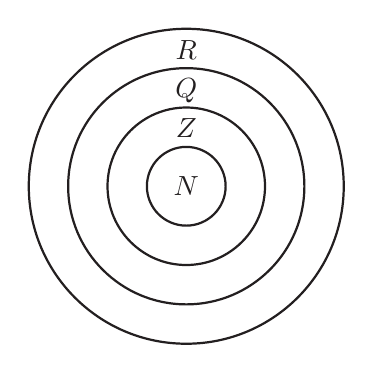
\begin{tikzpicture}
                    
                    \draw[black, thick] (0,0)   node[]                                    {$\mathbb{N}$} circle (0.5cm)
                                        (0,0.5) node[inner sep=1mm,anchor=center,above]   {$\mathbb{Z}$}
                                        (0,0)                                                            circle (1cm)
                                        (0,1)   node[inner sep=0.5mm,anchor=center,above] {$\mathbb{Q}$}
                                        (0,0)                                                            circle (1.5cm)
                                        (0,1.5) node[inner sep=1mm,anchor=center,above]   {$\mathbb{R}$}
                                        (0,0)                                                            circle (2cm);
                    
                \end{tikzpicture}
            \end{SummaryBox}
            
            \begin{SummaryBox}[title=Interval notation]
                \begin{itemize}[leftmargin=*]
                    \item Suppose that $a$ and $b$ are real numbers, with $a<b$.
                    \begin{multicols}{2}
                    \begin{itemize}[topsep=0pt]
                        \item $(a,b)      =\{x:a<    x<    b\}$
                        \item $[a,b]      =\{x:a\leq x\leq b\}$
                        \item $(a,b]      =\{x:a<    x\leq b\}$
                        \item $[a,b)      =\{x:a\leq x<    b\}$
                        \item $(a,\infty) =\{x:a<    x      \}$
                        \item $[a,\infty) =\{x:a\leq x      \}$
                        \item $(-\infty,b)=\{x:      x<    b\}$
                        \item $(-\infty,b]=\{x:a<    x\leq b\}$
                    \end{itemize}
                    \end{multicols}
                \end{itemize}
                \tcblower
                When using number lines to represent intervals,
                \begin{itemize}[topsep=0pt]
                    \item The `closed' circle ($\bullet$) indicates that the number is included.
                    \item The `open' circle ($\circ$) indicates that the number is \textbf{not} included.
                \end{itemize}
            \end{SummaryBox}
            
            \begin{SummaryBox}[title=Functions VS relations]
                \begin{itemize}[leftmargin=*]
                    \item A \textbf{function} is a relation such that for each $x$-value there is only one corresponding $y$-value. This means that, if $(a,b)$ and $(a,c)$ are ordered pairs of a function, then $b=c$.
                    \item In other words, a function cannot contain two different ordered pairs with the same first coordinate.
                \end{itemize}
                
                \begin{SummaryExtensionBox}[title=Vertical line test, center lower]
                    \begin{itemize}[leftmargin=*]
                        \item If a vertical line can be drawn anywhere on the graph and it only ever intersects the graph at a maximum of once, then the relation is a function.
                    \end{itemize}
                    \tcblower
                    \begin{tblr}{colspec={X[c]|X[c]}}
                        {\begin{tikzpicture}
                            \begin{axis}[
                                My Style 1,
                                xmin=-2,
                                xmax=2,
                                ymin=-2,
                                ymax=2
                            ]
                                \node[black, shift={(-2.5mm,-2.5mm)}, align=center] at (axis cs:0,0) {$O$};
                                \draw[black, thick] (axis cs:0,0) circle [radius=1];
                                \addplot+[black, thick, dashed, mark=none] coordinates {(0.5,-2) (0.5,2)};
                                \filldraw[black, thick] (axis cs:0.5,{-sqrt(3)/2}) circle [radius=2.5pt];
                                \filldraw[black, thick] (axis cs:0.5,{sqrt(3)/2}) circle [radius=2.5pt];
                            \end{axis}
                        \end{tikzpicture}\\
                        $x^2+y^2=1$ is not a function}
                        
                        &
                        
                        {\begin{tikzpicture}
                            \begin{axis}[
                                My Style 1,
                                xmin=-2,
                                xmax=2,
                                ymin=-2,
                                ymax=2
                            ]
                                \node[black, shift={(-2.5mm,-2.5mm)}, align=center] at (axis cs:0,0) {$O$};
                                \addplot[black, thick] {x^2};
                                \addplot+[black, thick, dashed, mark=none] coordinates {(0.5,-2) (0.5,2)};
                                \filldraw[black, thick] (axis cs:0.5,{0.5^2}) circle [radius=2.5pt];
                            \end{axis}
                        \end{tikzpicture}\\
                        $y=x^2$ is a function}
                    \end{tblr}
                \end{SummaryExtensionBox}
            \end{SummaryBox}
            
            \begin{SummaryBox}[title=Function notation]
                \[ \highmath{$ f:X \to Y, f(x) = \dots $} \]
                \begin{itemize}[leftmargin=*]
                    \item $f$ is the function name
                    \item $X$ is the \textbf{domain} of the function, \textit{i.e.,} the set of values for which the function is defined.
                    \item $Y$ is the \textbf{codomain} of the function, \textit{i.e.,} the set of values which the \textbf{range} (the range is the set of outputs of the function) of the function falls into.
                \end{itemize}
            \end{SummaryBox}
            
            \begin{SummaryBox}[title=Types of functions (many/one-to-one)]
                \begin{itemize}[leftmargin=*]
                    \item If $\forall a,b \in \dom(f): f(a) = f(b) \iff a = b$, or, to put it another way, $\forall a,b \in \dom(f): f(a) \neq f(b) \iff a \neq b$, then a function is a \textbf{one-to-one} function.
                    \item A function that does not satisfy the above condition(s) is a \textbf{many-to-one} function.
                \end{itemize}
                
                \begin{SummaryExtensionBox}[title=Horizontal line test, center lower]
                    \begin{itemize}[leftmargin=*]
                        \item If a horizontal line can be drawn anywhere on the graph of a function and it only ever intersects the graph a maximum of once, then the function is a \textbf{one-to-one}.
                    \end{itemize}
                    \tcblower
                    \begin{tblr}{colspec={X[c]|X[c]}}
                        {\begin{tikzpicture}
                            \begin{axis}[
                                My Style 1,
                                xmin=-2,
                                xmax=2,
                                ymin=-2,
                                ymax=2
                            ]
                                \node[black, shift={(-2.5mm,-2.5mm)}, align=center] at (axis cs:0,0) {$O$};
                                \addplot[black, thick] {x^2};
                                \addplot+[black, thick, dashed, mark=none] {1};
                                \filldraw[black, thick] (axis cs:-1,1) circle [radius=2.5pt];
                                \filldraw[black, thick] (axis cs:1,1) circle [radius=2.5pt];
                            \end{axis}
                        \end{tikzpicture}\\
                        $f(x)=x^2$ is a many-to-one function}
                        
                        &
                        
                        {\begin{tikzpicture}
                            \begin{axis}[
                                My Style 1,
                                xmin=-2,
                                xmax=2,
                                ymin=-2,
                                ymax=2
                            ]
                                \node[black, shift={(2.5mm,-2.5mm)}, align=center] at (axis cs:0,0) {$O$};
                                \addplot[black, thick] {x};
                                \addplot+[black, thick, dashed, mark=none] {1};
                                \filldraw[black, thick] (axis cs:1,1) circle [radius=2.5pt];
                            \end{axis}
                        \end{tikzpicture}\\
                        $f(x)=x$ is a one-to-one function}
                    \end{tblr}
                \end{SummaryExtensionBox}
            \end{SummaryBox}
            
            \begin{SummaryBox}[title=Parity of functions]
                \begin{itemize}[leftmargin=*]
                    \item A function is \textbf{even} if $\forall x \in \text{dom}(f): f(x) = f(-x)$.
                    \item A function is \textbf{odd} if $\forall x \in \text{dom}(f): f(-x) = -f(x)$.
                    \item A function can be \textbf{neither odd nor even} (if both of the above statements do not apply).
                \end{itemize}
            \end{SummaryBox}
            
            \begin{SummaryBox}[title=Implied/maximal domain]
                \begin{itemize}[leftmargin=*]
                    \item The \textbf{implied} domain (also referred to as the \textbf{maximal} domain) of a function is the largest subset of $\mathbb{R}$ for which the rule for the function is defined.
                \end{itemize}
            \end{SummaryBox}
            
            \begin{SummaryBox}[title=Sum and product of functions]
                \begin{itemize}[leftmargin=*]
                    \item $(f + g)(x) = f(x) + g(x)$ for $\dom(f) \cap \dom(g) \neq \varnothing$
                    \begin{itemize}[topsep=0pt]
                        \item $\dom(f + g) = \dom(f) \cap \dom(g)$
                    \end{itemize}
                    \item $(f - g)(x) = f(x) - g(x)$ for $\dom(f) \cap \dom(g) \neq \varnothing$
                    \begin{itemize}[topsep=0pt]
                        \item $\dom(f - g) = \dom(f) \cap \dom(g)$
                    \end{itemize}
                    \item $(f \cdot g)(x) = f(x) \cdot g(x)$ for $\dom(f) \cap \dom(g) \neq \varnothing$
                    \begin{itemize}[topsep=0pt]
                        \item $\dom(f \cdot g) = \dom(f) \cap \dom(g)$
                    \end{itemize}
                \end{itemize}
                
                \begin{SummaryExtensionBox}[title={Addition of ordinates (sketching \texorpdfstring{$\bm{y=(f + g)(x)}$}{$y=(f + g)(x)$})}, list text={Addition of ordinates (sketching $y=(f + g)(x)$)}]
                    \begin{itemize}[leftmargin=*]
                        \item When $f(x) = 0$, $(f + g)(x) = g(x)$.
                        \item When $g(x) = 0$, $(f + g)(x) = f(x)$.
                        \item If $f(x)$ and $g(x)$ are \textbf{both} positive, then $(f + g)(x) > f(x)$ \textbf{and} $(f + g)(x) > g(x)$.
                        \item If $f(x)$ and $g(x)$ are \textbf{both} negative, then $(f + g)(x) < f(x)$ \textbf{and} $(f + g)(x) < g(x)$.
                        \item If $f(x)$ is positive and $g(x)$ is negative, then $g(x) < (f + g)(x) < f(x)$.
                        \item Look for values of $x$ for which $f(x) + g(x) = 0$.
                    \end{itemize}
                \end{SummaryExtensionBox}
            \end{SummaryBox}
            
            \begin{SummaryBox}[title=Composite functions]
                \begin{itemize}[leftmargin=*]
                    \item Given that \highmath{$\ran(g) \subseteq \dom(f)$}, we can define the new function $h$ as a \textbf{composition} of $f$ with $g$.
                    \item This is written $h = f \circ g$ (read `composition of $g$ followed by $f$') and the rule for $h$ is given by $h(x) = f(g(x))$.
                    \begin{itemize}[topsep=0pt]
                        \item \highmath{\( \dom(h) = \curls*{ x \in \dom(g) : g(x) \in \dom(f) } \)}. In other words, the domain of \( h \) is the set of \( x \) such that \( x \in \dom(g) \), and using those \( x \)-values, the range of \( g(x) \) has to fit within the domain of \( f \) (because otherwise, \( f \) would be undefined for values that didn't belong in its domain).
                        \item \highmath{\( \ran(h) = f\pars*{ \ran(g) \cap \dom(f) } \)}. This is another way of saying that the range of \( h \) is the range of \( f(x) \) where \( x \in \dom(h) \).
                    \end{itemize}
                    \item Generally, \highmath{$f \circ g \neq g \circ f$}
                \end{itemize}
            \end{SummaryBox}
            
            \begin{SummaryBox}[title=Increasing and decreasing functions, leftlower=0pt, rightlower=0pt]
                \begin{itemize}[leftmargin=*]
                    \item If $\forall x \in \bracs*{x_1, x_2}: \highmath{$f\pars*{x_2} > f\pars*{x_1}$} \; \mid \; x_2 > x_1$, then $f$ is \textbf{strictly increasing} over the interval $\bracs*{x_1, x_2}$.
                    \item If $\forall x \in \bracs*{x_1, x_2}: \highmath{$f\pars*{x_2} < f\pars*{x_1}$} \; \mid \; x_2 > x_1$, then $f$ is \textbf{strictly decreasing} over the interval $\bracs*{x_1, x_2}$.
                    \item These intervals include the values of $x$ for which $\diff[f]{x}=0$, but the gradient never changes sign as such.
                    \begin{itemize}[topsep=0pt]
                        \item An example would be that the function of $f:[0,\infty) \to \mathbb{R}, f(x) = x^2$ is strictly increasing.
                    \end{itemize}
                    \item A function that is strictly increasing or decreasing is also a one-to-one function.
                \end{itemize}
                \tcblower
                \begin{tblr}{colspec={X[c]|X[c]}}
                    {\begin{tikzpicture}
                        \begin{axis}[
                            My Style 1,
                            xmin=-0.25,
                            xmax=2,
                            ymin=-0.25,
                            ymax=2,
                            extra x ticks={0.2,1.5},
                            extra x tick labels={$x_1$, $x_2$}
                        ]
                            \node[black, shift={(-2.5mm,-2.5mm)}, align=center] at (axis cs:0,0) {$O$};
                            \draw[black, thick] (axis cs:0.2,0.4) .. controls (axis cs:0.6, 1.2) and (axis cs:1.1,0.4) .. (axis cs:1.5, 1.75);
                        \end{axis}
                    \end{tikzpicture}\\
                    This function is \textbf{strictly increasing} over $\bracs*{x_1, x_2}$}
                    
                    &
                    
                    {\begin{tikzpicture}
                        \begin{axis}[
                            My Style 1,
                            xmin=-0.25,
                            xmax=2,
                            ymin=-0.25,
                            ymax=2,
                            extra x ticks={0.2,1.5},
                            extra x tick labels={$x_1$, $x_2$}
                        ]
                            \node[black, shift={(-2.5mm,-2.5mm)}, align=center] at (axis cs:0,0) {$O$};
                            \draw[black, thick] (axis cs:0.2,1.3) .. controls (axis cs:0.6, 1.2) and (axis cs:1.1,0.5) .. (axis cs:1.5, 0.4);
                        \end{axis}
                    \end{tikzpicture}\\
                    This function is \textbf{strictly decreasing} over $\bracs*{x_1, x_2}$}
                \end{tblr}
            \end{SummaryBox}
            
            \begin{SummaryBox}[title=Inverse functions, sidebyside, right=0pt, righthand ratio=0.45]
                \begin{itemize}
                    \item If $f$ is a \textbf{one-to-one function}, then a new function $f^{-1}$, called the \textbf{inverse} of $f$, may be defined by
                    \[
                        f^{-1}(x) = y\quad \text{if }f(y) = x,
                    \]
                    for $x \in \ran(f), y \in \dom(f)$.
                    \item Domain and range:
                    \begin{itemize}[topsep=0pt]
                        \item $\dom\pars*{f^{-1}} = \ran(f)$
                        \item $\ran\pars*{f^{-1}} = \dom(f)$
                    \end{itemize}
                    \item Compositions:
                    \begin{itemize}[topsep=0pt]
                        \item $\forall x \in \dom(f^{-1}): \pars*{f \circ f^{-1}}(x) = x$
                        \item $\forall x \in \dom(f): \pars*{f^{-1} \circ f}(x) = x$
                    \end{itemize}
                    \item The point $(x,y)$ is on the graph of $f^{-1}$ if and only if the point $(y,x)$ is on the graph of $f$. Thus, the graph of $f^{-1}$ is a \textbf{reflection} of the graph of $f$ in the line $y=x$.
                    \item If $f$ is strictly increasing, then $f^{-1}$ is also strictly increasing (and vice versa).
                    \item For a continuous function $f$ (and some non-continuous functions, too), \textbf{at least one} of the intersections of $f$ and $f^{-1}$ lie on the line $y=x$ (if the functions intersect at all, that is), so, to solve for this intersection point, either $f(x) = x$ or $f^{-1}(x) = x$ will suffice.
                    \begin{itemize}[topsep=0pt]
                        \item If ``just one intersection point'' is needed, then the line $y=x$ is \textbf{tangential} to both functions at that point. This means that the gradients of $f$, $f^{-1}$, and $y=x$ are equal at that point (they are all $1$, as the gradient of $y=x$ is always $1$).
                    \end{itemize}
                \end{itemize}
                \tcblower
                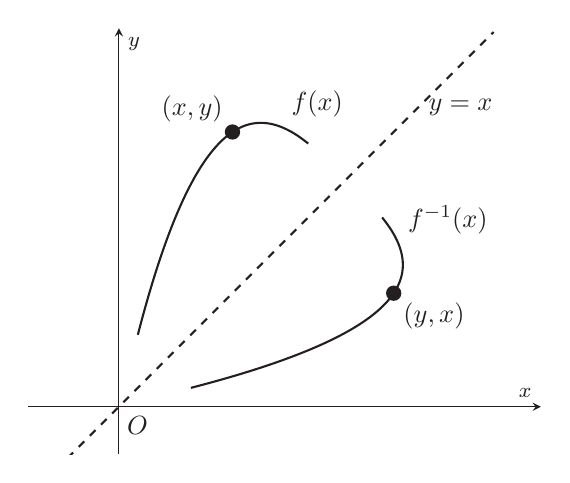
\begin{tikzpicture}[scale=0.95]
                    \begin{axis}[
                        My Style 1,
                        xmin=-0.25,
                        xmax=2,
                        ymin=-0.25,
                        ymax=2,
                        declare function={f(\x) = (\x-1)^2 * (\x-3);},
                        restrict y to domain=-2:2,
                    ]
                        \node[black, shift={(2.5mm,-2.5mm)}, align=center] at (axis cs:0,0) {$O$};
                        \addplot[black, thick, domain=0.1:1] {f(x+0.25)+1.5} node[pos=0.9, above right] {$f(x)$};
                        \addplot[black, thick, domain=0.1:1] ({f(x+0.25)+1.5}, x) node[pos=0.9, above right] {$f^{-1}(x)$};
                        \addplot+[black, thick, dashed, mark=none] {x} node[pos=0.9, right] {$y=x$};
                        \filldraw[black, thick] (axis cs:0.6,1.451625) circle [radius=2.5pt] node[above left] {$(x,y)$};
                        \filldraw[black, thick] (axis cs:1.451625,0.6) circle [radius=2.5pt] node[below right] {$(y,x)$};
                    \end{axis}
                \end{tikzpicture}
            \end{SummaryBox}
            
            \pagebreak
            
        \section{Coordinate geometry}
            
            \begin{SummaryBox}[title=Solving simultaneous equations]
                \begin{itemize}[leftmargin=*]
                    \item There are two ways to solve simultaneous equations: \textbf{substitution} and \textbf{elimination}.
                \end{itemize}
            \end{SummaryBox}
            
            \begin{SummaryBox}[title=Linear coordinate geometry, breakable]
                \begin{itemize}[leftmargin=*]
                    \item The following is revision of basic concepts of linear coordinate geometry.
                    \item This is \textbf{linear} coordinate geometry, meaning these concepts can only apply to straight lines.
                \end{itemize}
                
                \begin{SummaryExtensionBox}[title=Distance between two points, leftlower=0pt, rightlower=0pt]
                    \begin{itemize}[leftmargin=*]
                        \item Let $d$ be the \textbf{distance} between two points $A\pars*{x_1,y_1}$ and $B\pars*{x_2,y_2}$.
                        \[
                            d = \sqrt{ \pars*{x_2 - x_1}^2 + \pars*{y_2 - y_1}^2 }
                        \]
                    \end{itemize}
                    \tcblower
                    \begin{tblr}{colspec={X[c,h]|X[l,b]}}
                        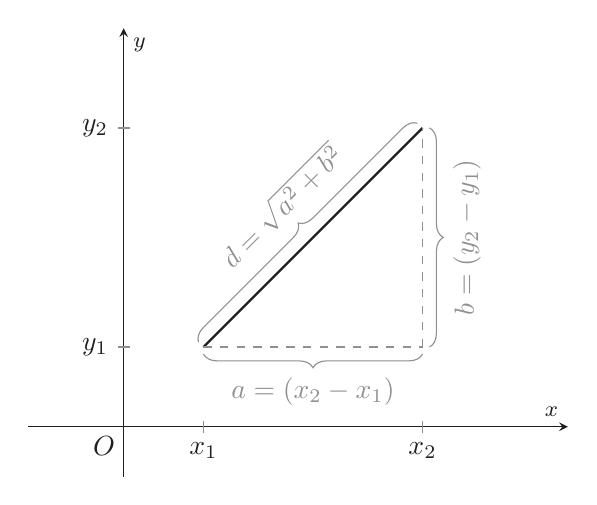
\begin{tikzpicture}[baseline=(current bounding box.north)]
                            \begin{axis}[
                                My Style 1,
                                xmin=-0.25,
                                xmax=2,
                                ymin=-0.25,
                                ymax=2,
                                extra x ticks={0.4,1.5},
                                extra x tick labels={$x_1$, $x_2$},
                                extra y ticks={0.4,1.5},
                                extra y tick labels={$y_1$, $y_2$},
                                clip=false
                            ]
                                \node[black, shift={(-2.5mm,-2.5mm)}, align=center] at (axis cs:0,0) {$O$};
                                \draw[black, thick] (axis cs:0.4,0.4) -- (axis cs:1.5,1.5);
                                \draw[gray, dashed] (axis cs:1.5,0.4) -- (axis cs:1.5,1.5);
                                \draw[gray, decorate, decoration={brace,amplitude=5pt,mirror,raise=2.5}] (axis cs:1.5,0.4) -- (axis cs:1.5,1.5) node[midway, sloped, below, yshift=(-5pt - 2.5)] {$b = \pars*{y_2 - y_1}$};
                                \draw[gray, dashed] (axis cs:0.4,0.4) -- (axis cs:1.5,0.4);
                                \draw[gray, decorate, decoration={brace,amplitude=5pt,mirror,raise=2.5}] (axis cs:0.4,0.4) -- (axis cs:1.5,0.4) node[midway, below, yshift=(-5pt - 2.5)] {$a = \pars*{x_2 - x_1}$};
                                \draw[gray, decorate, decoration={brace,amplitude=5pt,raise=2.5}] (axis cs:0.4,0.4) -- (axis cs:1.5,1.5) node[midway, sloped, above, yshift=(5pt + 2.5)] {$d = \sqrt{a^2 + b^2}$};
                            \end{axis}
                        \end{tikzpicture}
                        &
                        The Pythagorean theorem comes into play for the derivation of the distance formula, as it is just the hypotenuse of a right-angled triangle formed by the horizontal and vertical components of the line.
                    \end{tblr}
                \end{SummaryExtensionBox}
                
                \begin{SummaryExtensionBox}[title=Midpoint of a line]
                    \begin{itemize}[leftmargin=*]
                        \item The \textbf{midpoint}, of a line beginning and ending at points $A\pars*{x_1,y_1}$ and $B\pars*{x_2,y_2}$ respectively is given by the formula:
                        \[
                            \text{Midpoint} = \pars*{ \frac{x_1 + x_2}{2}, \frac{y_1 + y_2}{2} }
                        \]
                    \end{itemize}
                \end{SummaryExtensionBox}
                
                \begin{SummaryExtensionBox}[title=Gradient of a line]
                    \begin{itemize}[leftmargin=*]
                        \item The \textbf{gradient}, $m$, of a line going through the points $A\pars*{x_1,y_1}$ and $B\pars*{x_2,y_2}$ is given by the formula:
                        \[
                            m = \frac{y_2 - y_1}{x_2 - x_1}
                        \]
                    \end{itemize}
                \end{SummaryExtensionBox}
                
                \begin{SummaryExtensionBox}[title=Equation of a line]
                    \begin{itemize}[leftmargin=*]
                        \item The equation of a line (in slope-intercept form) with a $y$-intercept at the point $A\pars*{0,c}$ is given by the formula:
                        \[
                            y = mx + c
                        \]
                        \item The equation of a line (in point-slope form) going through the point $A\pars*{x_1,y_1}$ is given by the formula:
                        \[
                            y - y_1 = m\pars*{x-x_1}
                        \]
                        \item The equation of a line (in intercept form) going through the two points $A\pars*{a,0}$ and $B\pars*{0,b}$ is given by the formula:
                        \[
                            \frac{x}{a} + \frac{y}{b} = 1
                        \]
                    \end{itemize}
                \end{SummaryExtensionBox}
                
                \begin{SummaryExtensionBox}[title=Tangent of the angle of slope, sidebyside, lefthand ratio=0.45]
                    \begin{itemize}[leftmargin=*]
                        \item For a straight line with gradient $m$, the angle of slope is found using:
                        \[
                            m = \tan(\theta)
                        \]
                        where $\theta$ is the angle that the line makes with the positive direction of the $x$-axis.
                    \end{itemize}
                    \tcblower
                    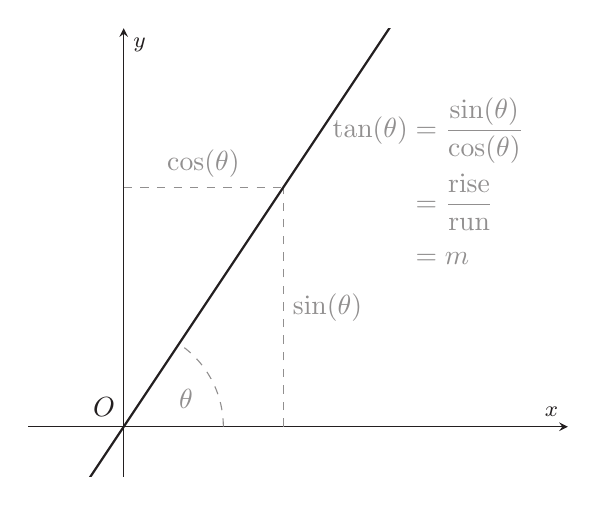
\begin{tikzpicture}
                        \begin{axis}[
                            My Style 1,
                            xmin=-0.25,
                            xmax=2,
                            ymin=-0.25,
                            ymax=2,
                            declare function={f(\x)=1.5*\x;}
                        ]
                            \node[black, shift={(-2.5mm,2.5mm)}, align=center] at (axis cs:0,0) {$O$};
                            \draw[gray, dashed] (axis cs:0.5,0) arc[start angle=0, end angle=(atan(1.5)), radius=0.5] node[left, yshift=-7mm, xshift=3mm] {$\theta$};
                            \draw[gray, dashed] (axis cs:0.8,0) -- (axis cs:0.8,{f(0.8)}) node[right, midway] {$\sin(\theta)$};
                            \draw[gray, dashed] (axis cs:0,{f(0.8)}) -- (axis cs:0.8,{f(0.8)}) node[above, midway] {$\cos(\theta)$};
                            \node[gray, anchor=north west] at (axis cs:1,1.7) {$\begin{aligned} \tan(\theta) &= \frac{\sin(\theta)}{\cos(\theta)} \\ &= \frac{\text{rise}}{\text{run}} \\ &= m \end{aligned}$};
                            \addplot[black, thick] {f(x)};
                        \end{axis}
                    \end{tikzpicture}
                \end{SummaryExtensionBox}
                
                \begin{SummaryExtensionBox}[title=Perpendicular and parallel lines]
                    \begin{itemize}[leftmargin=*]
                        \item If two straight lines are perpendicular to each other (meet at right angles), the product of their gradients is $-1$ (unless one is vertical and the other horizontal).
                        \[
                            m_\perp \times m = -1
                        \]
                        \item Parallel lines have the same gradient.
                    \end{itemize}
                \end{SummaryExtensionBox}
            \end{SummaryBox}
            
            \begin{SummaryBox}[title=The geometry of simultaneous linear equations, leftlower=0pt, rightlower=0pt]
                \begin{itemize}[leftmargin=*]
                    \item There are three cases for a system of two linear equations with two variables.
                \end{itemize}
                \tcblower
                \begin{tblr}{colspec={X[r,m,0.1,font=\itshape]|X[c,0.25]|X[l,0.3]|X[l,0.35]}, rowspec={Q[c,font=\bfseries]|Q|Q|Q}}
                             &    Example                                                        &    Solutions                              &    Geometry    \\
                   Case 1    &    $\begin{aligned}[t] 2x+y &= 5 \\ x-y &= 4 \end{aligned}$       &    {Unique solution: \\ $x=3$, $y=-1$}    &    Two lines meeting at a point \\
                   Case 2    &    $\begin{aligned}[t] 2x+y &= 5 \\ 2x+y &= 7 \end{aligned}$      &    No solutions                           &    Distinct parallel lines \\
                   Case 3    &    $\begin{aligned}[t] 2x+y &= 5 \\ 4x+2y &= 10 \end{aligned}$    &    Infinitely many solutions              &    Two copies of the same line
                \end{tblr}
            \end{SummaryBox}
            
            \begin{SummaryBox}[title=Transformations, breakable]
                \begin{SummaryExtensionBox}[title=Dilations, leftlower=0pt, rightlower=0pt]
                    \begin{itemize}[leftmargin=*]
                        \item Dilation from the $x$-axis:
                        \begin{itemize}[topsep=0pt]
                            \item For $b \in \mathbb{R}^+$, a dilation of factor $b$ from the $x$-axis is described by the rule:
                            \[
                                \pars*{x,y} \to \pars*{x,by}
                            \]
                            \item This means that this dilation can also be applied as such: $y=b \cdot f(x)$.
                        \end{itemize}
                        \item Dilation from the $y$-axis:
                        \begin{itemize}[topsep=0pt]
                            \item For $a \in \mathbb{R}^+$, a dilation of factor $a$ from the $y$-axis is described by the rule:
                            \[
                                \pars*{x,y} \to \pars*{ax,y}
                            \]
                            \item This means that this dilation can also be applied as such: $y=f\pars*{\frac{x}{a}}$.
                        \end{itemize}
                    \end{itemize}
                    \tcblower
                    \begin{tblr}{colspec={X[r,m,0.07] | X[c,0.465] | X[c,0.465]}, hline{2-Y}}
                        From             &    factor $2$    &    factor $\frac{1}{2}$    \\
                        $x$-axis         &    {   \begin{tikzpicture}[baseline=(current bounding box).north]
                                                      \begin{axis}[
                                                          My Style 1,
                                                          xmin=-0.25,
                                                          xmax=1.5,
                                                          ymin=-0.25,
                                                          ymax=1.5,
                                                          width=\linewidth
                                                      ]
                                                          \node[black, shift={(2.5mm,-2.5mm)}, align=center] at (axis cs:0,0) {$O$};
                                                          \addplot[black, thick, dashed, domain=0:1.5] {sqrt(x)} node[pos=0.6, below right, inner sep=0pt] {$y=\sqrt{x}$};
                                                          \addplot[black, thick, domain=0:1.5] {2*sqrt(x)} node[pos=0.45, below right, inner sep=0pt] {$y=2\sqrt{x}$};
                                                      \end{axis}
                                                  \end{tikzpicture}}    &    {   \begin{tikzpicture}[baseline=(current bounding box).north]
                                                                                 \begin{axis}[
                                                                                     My Style 1,
                                                                                     xmin=-0.25,
                                                                                     xmax=1.5,
                                                                                     ymin=-0.25,
                                                                                     ymax=1.5,
                                                                                     width=\linewidth
                                                                                 ]
                                                                                     \node[black, shift={(2.5mm,-2.5mm)}, align=center] at (axis cs:0,0) {$O$};
                                                                                     \addplot[black, thick, dashed, domain=0:1.5] {sqrt(x)} node[pos=0.6, above left, inner sep=0pt] {$y=\sqrt{x}$};
                                                                                     \addplot[black, thick, domain=0:1.5] {(1/2)*sqrt(x)} node[pos=0.6, below right, inner sep=0pt] {$y=\frac{1}{2}\sqrt{x}$};
                                                                                  \end{axis}
                                                                                  \end{tikzpicture}}                   \\
                        $y$-axis         &    {   \begin{tikzpicture}[baseline=(current bounding box).north]
                                                      \begin{axis}[
                                                          My Style 1,
                                                          xmin=-0.25,
                                                          xmax=1.5,
                                                          ymin=-0.25,
                                                          ymax=1.5,
                                                          width=\linewidth
                                                      ]
                                                          \node[black, shift={(2.5mm,-2.5mm)}, align=center] at (axis cs:0,0) {$O$};
                                                          \addplot[black, thick, dashed, domain=0:1.5] {sqrt(x)} node[pos=0.6, above left, inner sep=0pt] {$y=\sqrt{x}$};
                                                          \addplot[black, thick, domain=0:1.5] {sqrt(x/2)} node[pos=0.45, below right, inner sep=0pt] {$y=\sqrt{\frac{x}{2}}$};
                                                      \end{axis}
                                                  \end{tikzpicture}}    &    {   \begin{tikzpicture}[baseline=(current bounding box).north]
                                                                                 \begin{axis}[
                                                                                     My Style 1,
                                                                                     xmin=-0.25,
                                                                                     xmax=1.5,
                                                                                     ymin=-0.25,
                                                                                     ymax=1.5,
                                                                                     width=\linewidth
                                                                                 ]
                                                                                     \node[black, shift={(2.5mm,-2.5mm)}, align=center] at (axis cs:0,0) {$O$};
                                                                                     \addplot[black, thick, dashed, domain=0:1.5] {sqrt(x)} node[pos=0.6, below right, inner sep=0pt] {$y=\sqrt{x}$};
                                                                                     \addplot[black, thick, domain=0:1.5] {sqrt(x/(1/2))} node[pos=0.775, below right, inner sep=0pt, scale=0.9] {$y=\sqrt{2x}$};
                                                                                  \end{axis}
                                                                                  \end{tikzpicture}}
                    \end{tblr}
                \end{SummaryExtensionBox}
                
                \begin{SummaryExtensionBox}[title=Table of transformations, left=0pt, right=0pt]
                    \begin{tblr}{colspec={X[l,m,0.6] | X[c,m,0.2,mode=dmath] | X[c,m,0.2,mode=dmath]}, hline{2-Y}, row{1}={c,font=\bfseries\large}}
                        Mapping                                                               &    \bm{(x,y)\to{}}    &    \bm{y=f(x)\to{}}          \\
                        Reflection in the $x$-axis                                            &    \pars*{x,-y}       &    y=-f(x)                   \\
                        Reflection in the $y$-axis                                            &    \pars*{-x,y}       &    y=f(-x)                   \\
                        Dilation of factor $a$ from the $y$-axis                              &    \pars*{ax,y}       &    y=f\pars*{\frac{x}{a}}    \\
                        Dilation of factor $b$ from the $x$-axis                              &    \pars*{x,by}       &    y=bf(x)                   \\
                        Reflection in the line $y=x$ (inverse function)                       &    \pars*{y,x}        &    x=f(y)                    \\
                        Translation of $h$ units in the positive direction of the $x$-axis    &    \pars*{x+h,y}      &    y=f(x-h)                  \\
                        Translation of $k$ units in the positive direction of the $y$-axis    &    \pars*{x,y+k}      &    y-k=f(x)
                    \end{tblr}
                \end{SummaryExtensionBox}
                
                \begin{SummaryExtensionBox}[title=Applying transformations]
                    \begin{enumerate}[leftmargin=*]
                        \item $T:\mathbb{R}^2 \to \mathbb{R}^2, T\pars*{x,y} = \pars*{ax+h, by+k},\quad a \neq 0, b \neq 0 $
                        \begin{itemize}[topsep=0pt]
                            \item Note that this notation is the same as writing $\pars*{x,y} \to \pars*{ax+h, by+k}$.
                        \end{itemize}
                        \item Denote the \textbf{transformed} pair of coordinates (the new ones) as $\pars*{x', y'}$.
                        \item $\begin{aligned}[t]
                                  \pars*{x', y'} &= T\pars*{x,y} \\
                                  \therefore \pars*{x', y'} &= \pars*{ax+h, by+k},\quad a \neq 0, b \neq 0
                               \end{aligned}$
                        \item Solve for the original $x$ and $y$ to be subbed into the function in question.\\
                        $\begin{aligned}[t]
                            x' &= ax + h \\
                            \therefore x &= \frac{x' - h}{a} \\[\belowdisplayskip]
                            %
                            y' &= bx + k \\
                            \therefore y &= \frac{y' - k}{b}
                         \end{aligned}$
                         \item Substitute $x$ and $y$ back into the function $y=f(x)$.
                         \begin{itemize}[topsep=0pt]
                             \item Remember to solve for $y$ if there is more than one term on that side of the equation.
                         \end{itemize}
                    \end{enumerate}
                \end{SummaryExtensionBox}
            \end{SummaryBox}
            
            \pagebreak
            
        \section{Polynomial functions}
            
            \begin{SummaryBox}[title=Quadratics]
                \begin{itemize}[leftmargin=*]
                    \item For a quadratic in standard (polynomial) form $\pars*{ax^2 + bx + c}$,
                    \begin{itemize}[topsep=0pt]
                        \item if $a>0$, then the graph has a \textbf{minimum} point.
                        \item if $a<0$, then the graph has a \textbf{maximum} point.
                        \item the \textbf{vertex} (\textbf{turning point}) is the point $(h,k)$, where $h=-\frac{b}{2a}$ and $k=\frac{4ac-b^2}{4a}$.
                        \item the \textbf{axis of symmetry} is $x=h$, where $h=-\frac{b}{2a}$.
                        \item the quadratic can be written in ``turning point form'' by \textbf{completing the square} for $x$ using the formula:
                        \[
                            ax^2 + bx + c = a\pars*{x+\frac{b}{2a}}^2 + \frac{4ac-b^2}{4a}
                        \]
                        \item the solutions to $ax^2 + bx + c = 0$ can be obtained using the \textbf{quadratic formula}:
                        \[
                            x = \frac{-b \pm \sqrt{b^2 - 4ac}}{2a}, \quad a \neq 0
                        \]
                        \item the \textbf{discriminant} ($\Delta$) for a quadratic polynomial is:
                        \[
                            \Delta = b^2 - 4ac
                        \]
                        For the equation $ax^2 + bx + c = 0$,
                        \begin{itemize}[topsep=0pt]
                            \item if $\Delta > 0$, there are two solutions.
                            \item if $\Delta = 0$, there is one solution (tangential).
                            \item if $\Delta < 0$, there are no solutions.
                        \end{itemize}
                        For the equation $ax^2 + bx + c = 0$ where $a,b,c \in \mathbb{Q}$,
                        \begin{itemize}[topsep=0pt]
                            \item if $\Delta$ is a perfect square and $\Delta \neq 0$, then the equation has two rational solutions.
                            \item if $\Delta = 0$, then the equation has one rational solution.
                            \item if $\Delta$ is not a perfect square and $\Delta > 0$, then the equation has two irrational solutions.
                        \end{itemize}
                    \end{itemize}
                \end{itemize}
            \end{SummaryBox}
            
            \begin{SummaryBox}[title=Remainder theorem]
                \begin{itemize}[leftmargin=*]
                    \item When $P(x)$ is divided by $\beta x + \alpha$, the remainder is $P\pars*{-\frac{\alpha}{\beta}}$.
                \end{itemize}
            \end{SummaryBox}
            
            \begin{SummaryBox}[title=Factor theorem]
                \begin{itemize}[leftmargin=*]
                    \item For the polynomial $P(x)$, if $P(\alpha) = 0$, then $x-\alpha$ is a factor of $P(x)$.
                    \item Conversely, if $x-\alpha$ is a factor of $P(x)$, then $P(\alpha) = 0$.
                \end{itemize}
                
                More generally:
                \begin{itemize}[leftmargin=*]
                    \item For the polynomial $P(x)$, if $\beta x + \alpha$ is a factor of $P(x)$, then $P\pars*{-\frac{\alpha}{\beta}} = 0$.
                    \item Conversely, if $P\pars*{-\frac{\alpha}{\beta}} = 0$, then $\beta x + \alpha$ is a factor of $P(x)$.
                \end{itemize}
            \end{SummaryBox}
            
            \begin{SummaryBox}[title=Rational root theorem]
                \begin{itemize}[leftmargin=*]
                    \item The root of a polynomial function $P(x)$ such that:
                    \[
                        P(x) = a_nx^n + a_{n-1}x^{n-1} + \dots + a_2x^2 + a_1x + a_0
                    \]
                    where the coefficients are integers is of the form:
                    \[
                        \frac{p}{q},\text{ where }p = \text{a factor of }a_0\text{ and }q = \text{a factor of }a_n
                    \]
                \end{itemize}
            \end{SummaryBox}
            
            \begin{SummaryBox}[title=Polynomials of degree \texorpdfstring{$\bm{n}$}{$n$}, list text={Polynomials of degree $n$}]
                \begin{itemize}[leftmargin=*]
                    \item For a polynomial $P(x)$ of degree $n$, there are \textbf{at most} $n$ solutions to the equation $P(x)=0$. Therefore, the graph of $P(x)$ has \textbf{at most} $n$ $x$-axis intercepts.
                    \item The graph of a polynomial of even degree may have no $x$-axis intercepts: for example, $P(x) = x^2 + 1$. But the graph of a polynomial of odd degree must have at least one $x$-axis intercept.
                \end{itemize}
            \end{SummaryBox}
            
            \begin{SummaryBox}[title=Difference and sum of two variables of the same degree]
                \begin{itemize}[leftmargin=*]
                    \item $x^2 - y^2 = (x-y)(x+y)$
                    \item $x^3 - y^3 = (x+y)\pars*{x^2 - xy + y^2}$
                    \item If $n$ is odd,
                    \begin{itemize}[topsep=0pt]
                        \item $x^n - y^n = (x-y)\pars*{x^{n-1} + x^{n-2}y + \dots + xy^{n-2} + y^{n-1}}$
                        \item $x^n + y^n = (x+y)\pars*{x^{n-1} - x^{n-2}y + \dots + xy^{n-2} + y^{n-1}}$
                    \end{itemize}
                \end{itemize}
            \end{SummaryBox}
            
            \pagebreak
        
        \section{Exponential functions}
            
            \begin{SummaryBox}[title=Exponential function characteristics]
                \begin{itemize}[leftmargin=*]
                    \item For $a \in \mathbb{R}^+ \setminus \curls{1}$, the graph of $y=a^x$ has the following properties:
                    \begin{multicols}{2}
                        \begin{itemize}[topsep=0pt]
                            \item The $x$-axis is an asymptote.
                            \item The $y$-values are always positive.
                            \item The $y$-axis intercept is $1$.
                            \item There is no $x$-axis intercept.
                        \end{itemize}
                    \end{multicols}
                \end{itemize}
            \end{SummaryBox}
            
            \begin{SummaryBox}[title=Euler's number --- \texorpdfstring{$\bm{e}$}{$e$}, list text={Euler's number --- $e$}]
                \begin{itemize}[leftmargin=*]
                    \item Euler's number is defined as follows:
                    \[
                        e = \lim\limits_{n \to \infty} \pars*{1+\frac{1}{n}}^n = \num{2.718281828}\dots
                    \]
                \end{itemize}
            \end{SummaryBox}
            
            \begin{SummaryBox}[title=Index laws]
                For all positive numbers $a$ and $b$ and all real numbers $x$ and $y$:
                
                \vspace{10pt}
                \begin{tblr}{colspec={*{4}{X[l,m,mode=dmath]}}}
                    \text{\scriptsize\raisebox{0.35ex}{$\blacksquare$}\hspace{10pt}} a^x \cdot a^y = a^{x+y} &
                    \text{\scriptsize\raisebox{0.35ex}{$\blacksquare$}\hspace{10pt}} a^x \div a^y = a^{x-y} &
                    \text{\scriptsize\raisebox{0.35ex}{$\blacksquare$}\hspace{10pt}} \pars*{a^x}^y = a^{xy} &
                    \text{\scriptsize\raisebox{0.35ex}{$\blacksquare$}\hspace{10pt}} (ab)^x = a^xb^x \\
                    \text{\scriptsize\raisebox{0.35ex}{$\blacksquare$}\hspace{10pt}} \pars*{\frac{a}{b}}^x = \frac{a^x}{b^x} &
                    \text{\scriptsize\raisebox{0.35ex}{$\blacksquare$}\hspace{10pt}} a^{-x} = \frac{1}{a} &
                    \text{\scriptsize\raisebox{0.35ex}{$\blacksquare$}\hspace{10pt}} a^x = \frac{1}{a^{-x}} &
                    \text{\scriptsize\raisebox{0.35ex}{$\blacksquare$}\hspace{10pt}} a^0 = 1
                \end{tblr}
            \end{SummaryBox}
            
            \begin{SummaryBox}[title=Logarithms]
                \begin{itemize}[leftmargin=*]
                    \item For $a \in \mathbb{R}^+ \setminus \curls{1}$, the \textbf{logarithm function} with base $a$ is defined as follows:
                    \[
                        a^x = y \iff \log\limits_a (y) = x
                    \]
                    \item Since $a$ is positive, the expression $\log\limits_a (y)$ is only defined when $y$ is positive ($y>0$).
                \end{itemize}
                
                \begin{SummaryExtensionBox}[title=Log laws]
                    \begin{multicols}{2}
                        \begin{itemize}[leftmargin=*, itemsep=5pt]
                            \item $\log\limits_a (1) = 0$
                            \item $\log\limits_a (a) = 1$
                            \item $\log\limits_a \pars*{x^b} = b \cdot \log\limits_a (x)$
                            \item $\log\limits_{a^b} (x) = \frac{1}{b} \cdot \log\limits_a (x)$
                            \item $\log\limits_a \pars*{\frac{1}{x}} = -\log\limits_a (x)$
                            \item $\log\limits_{\frac{1}{a}} (x) = -\log\limits_a (x)$
                            \item $\log\limits_a (b) = \frac{\ln(b)}{\ln(a)}$
                            \item $\log\limits_a \pars*{a^b} = b$
                            \item $\log\limits_a \bracs*{\pars*{\frac{1}{a}}^n} = -n$
                            \item $a^{\log\limits_a \pars*{b}} = b$
                            \item $\log\limits_a (a) + \log\limits_a (b) = \log\limits_a (ab)$
                            \item $\log\limits_a (a) - \log\limits_a (b) = \log\limits_a \pars*{\frac{a}{b}}$
                        \end{itemize}
                    \end{multicols}
                \end{SummaryExtensionBox}
                
                \begin{itemize}[leftmargin=*]
                    \item The graph of $y=\log\limits_a (x)$ can be obtained from the graph of $y=\log\limits_b (x)$ by a dilation of factor $\frac{1}{\log\limits_b (a)}$ from the $x$-axis.
                    \item The graph of $y=a^x$ can be obtained from the graph of $y=b^x$ by a dilation of factor $\frac{1}{\log\limits_b (a)}$ from the $y$-axis.
                    \item When dividing both sides of an inequality by $\log\limits_a (x)$ where $0<x<1$, reverse the inequality as the logarithm will evaluate to negative.
                \end{itemize}
            \end{SummaryBox}
            
            \begin{SummaryBox}[title=Exponential growth and decay]
                \begin{itemize}[leftmargin=*]
                    \item In a situation where the growth/decay of something is exponential, the amount of that thing can be modelled using a function of the form:
                    \[
                        A(t) = A_0 \cdot e^{kt}
                    \]
                    where $A_0$ is the initial quantity at $t=0$ (where $t$ is a variable representing a unit of time) and $k$ is a constant.
                    \begin{itemize}[topsep=0pt]
                        \item Growth corresponds to $k>0$.
                        \item Decay corresponds to $k<0$.
                    \end{itemize}
                \end{itemize}
            \end{SummaryBox}
            
            \pagebreak
            
        \section{Circular functions}
            
            \begin{SummaryBox}[title=Radians and degrees]
                \begin{itemize}[leftmargin=*]
                    \item One \textbf{radian} (written $1^c$) is the angle subtended at the centre of the unit circle by an arc of length 1 unit.
                    \item To convert between the two, use the following:
                    \[
                        1^c = \frac{180^\circ}{\pi} \quad \text{or} \quad 1^\circ = \frac{\pi^c}{180}
                    \]
                \end{itemize}
            \end{SummaryBox}
            
            \begin{SummaryBox}[title=Unit circle, center upper, left=0pt, right=0pt]
                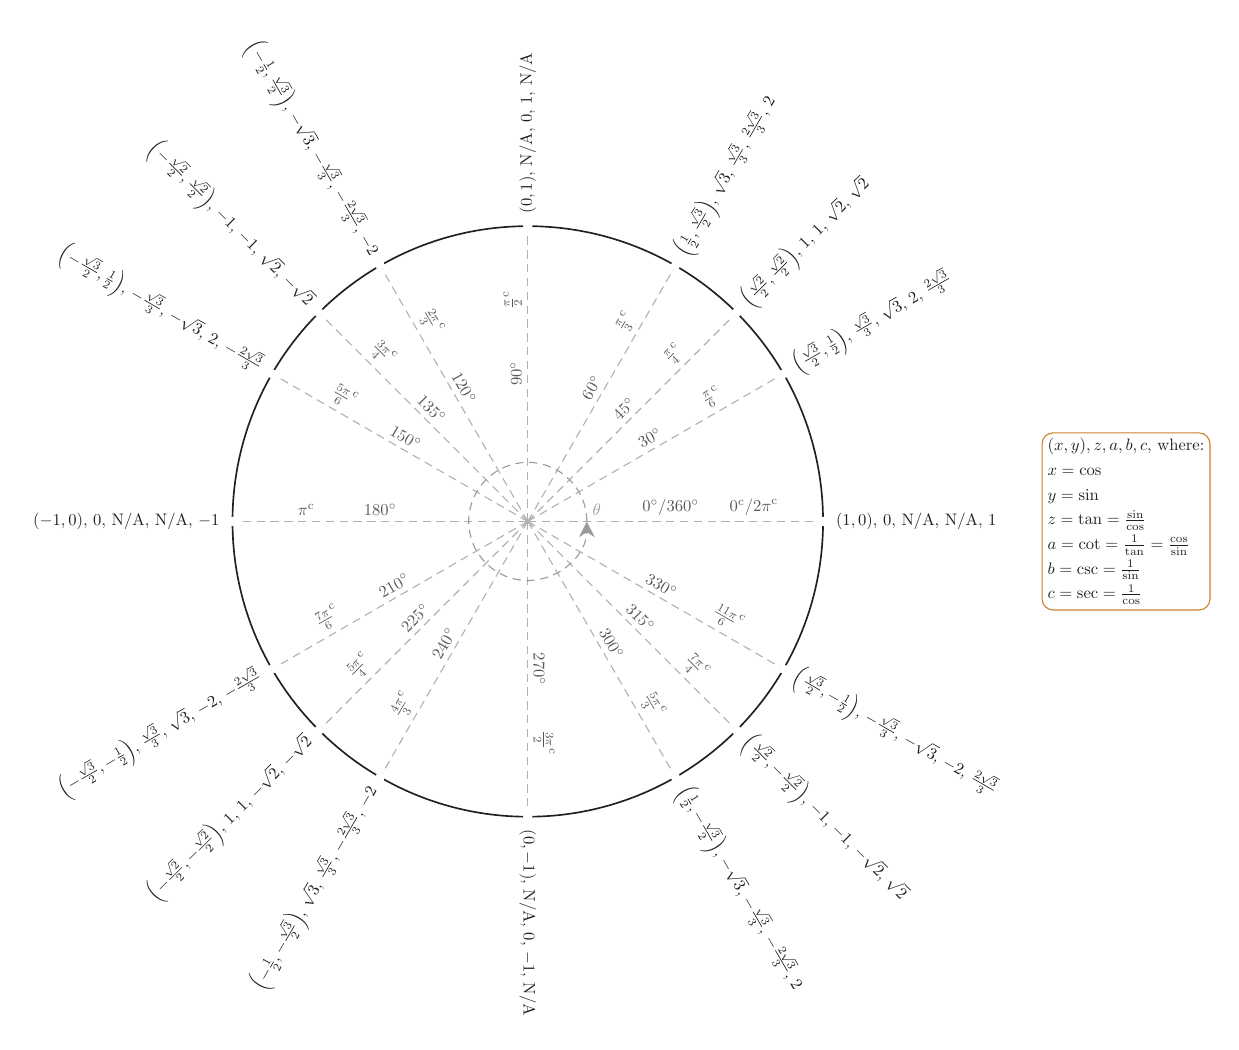
\begin{tikzpicture}
                    [
                        angle line/.style       = {white!65!black, thin, densely dashed},
                        angle dot/.style        = {fill=white, circle, minimum size=2mm, inner sep=0, pos=1},
                        angle num deg/.style    = {pos=0.5, sloped, above, white!25!black},
                        angle num rad/.style    = {pos=0.75, sloped, above, white!25!black},
                        angle inf right/.style  = {pos=1, sloped, right, anchor=west, shift={(0.15,0)}, black},
                        angle inf left/.style   = {pos=1, sloped, right, anchor=east, shift={(-0.15,0)}, black},
                        scale                   = 0.75,
                        every node/.style       = {scale=0.6}
                    ]

                    \draw[black, semithick] (0,0) circle [radius=5];


                    %                                                                          ANGLE (DEG)                                      ANGLE (RAD)                                                             COSINE                          SINE                            TANGENT                 COTANGENT               COSECANT                SECANT
                    \draw[angle line] (0,0) -- (0:5)    node[angle dot] {} node[angle num deg, xshift=-1mm] {$0^{\circ}/360^{\circ}$} node[angle num rad, xshift=1mm]    {$0^{\text{c}}/{2\pi}^{\text{c}}$} node[angle inf right]    (0-2pi)     {$\left(1,                      0\right)$,                      $0$,                    N/A,                    N/A,                    $1$};

                    \draw[angle line] (0,0) -- (30:5)   node[angle dot] {} node[angle num deg] {$30^{\circ}$}   node[angle num rad]             {${\frac{\pi}{6}}^{\text{c}}$}      node[angle inf right]   (pi_6)      {$\left(\frac{\sqrt{3}}{2},     \frac{1}{2}\right)$,            $\frac{\sqrt{3}}{3}$,   $\sqrt{3}$,             $2$,                    $\frac{2\sqrt{3}}{3}$};
                    \draw[angle line] (0,0) -- (45:5)   node[angle dot] {} node[angle num deg] {$45^{\circ}$}   node[angle num rad]             {${\frac{\pi}{4}}^{\text{c}}$}      node[angle inf right]   (pi_4)      {$\left(\frac{\sqrt{2}}{2},     \frac{\sqrt{2}}{2}\right)$,     $1$,                    $1$,                    $\sqrt{2}$,             $\sqrt{2}$};
                    \draw[angle line] (0,0) -- (60:5)   node[angle dot] {} node[angle num deg] {$60^{\circ}$}   node[angle num rad]             {${\frac{\pi}{3}}^{\text{c}}$}      node[angle inf right]   (pi_3)      {$\left(\frac{1}{2},            \frac{\sqrt{3}}{2}\right)$,     $\sqrt{3}$,             $\frac{\sqrt{3}}{3}$,   $\frac{2\sqrt{3}}{3}$,  $2$};

                    \draw[angle line] (0,0) -- (90:5)   node[angle dot] {} node[angle num deg] {$90^{\circ}$}   node[angle num rad]             {${\frac{\pi}{2}}^{\text{c}}$}      node[angle inf right]   (pi_2)      {$\left(0,                      1\right)$,                      N/A,                    $0$,                    $1$,                    N/A};

                    \draw[angle line] (0,0) -- (120:5)  node[angle dot] {} node[angle num deg] {$120^{\circ}$}  node[angle num rad]             {${\frac{2\pi}{3}}^{\text{c}}$}     node[angle inf left]    (2pi_3)     {$\left(-\frac{1}{2},           \frac{\sqrt{3}}{2}\right)$,     $-\sqrt{3}$,            $-\frac{\sqrt{3}}{3}$,  $-\frac{2\sqrt{3}}{3}$, $-2$};
                    \draw[angle line] (0,0) -- (135:5)  node[angle dot] {} node[angle num deg] {$135^{\circ}$}  node[angle num rad]             {${\frac{3\pi}{4}}^{\text{c}}$}     node[angle inf left]    (3pi_4)     {$\left(-\frac{\sqrt{2}}{2},    \frac{\sqrt{2}}{2}\right)$,     $-1$,                   $-1$,                   $\sqrt{2}$,             $-\sqrt{2}$};
                    \draw[angle line] (0,0) -- (150:5)  node[angle dot] {} node[angle num deg] {$150^{\circ}$}  node[angle num rad]             {${\frac{5\pi}{6}}^{\text{c}}$}     node[angle inf left]    (5pi_6)     {$\left(-\frac{\sqrt{3}}{2},    \frac{1}{2}\right)$,            $-\frac{\sqrt{3}}{3}$,  $-\sqrt{3}$,            $2$,                    $-\frac{2\sqrt{3}}{3}$};

                    \draw[angle line] (0,0) -- (180:5)  node[angle dot] {} node[angle num deg] {$180^{\circ}$}  node[angle num rad]             {${\pi}^{\text{c}}$}                node[angle inf left]    (pi)        {$\left(-1,                     0\right)$,                      $0$,                    N/A,                    N/A,                    $-1$};

                    \draw[angle line] (0,0) -- (210:5)  node[angle dot] {} node[angle num deg] {$210^{\circ}$}  node[angle num rad]             {${\frac{7\pi}{6}}^{\text{c}}$}     node[angle inf left]    (7pi_6)     {$\left(-\frac{\sqrt{3}}{2},    -\frac{1}{2}\right)$,           $\frac{\sqrt{3}}{3}$,   $\sqrt{3}$,             $-2$,                   $-\frac{2\sqrt{3}}{3}$};
                    \draw[angle line] (0,0) -- (225:5)  node[angle dot] {} node[angle num deg] {$225^{\circ}$}  node[angle num rad]             {${\frac{5\pi}{4}}^{\text{c}}$}     node[angle inf left]    (5pi_4)     {$\left(-\frac{\sqrt{2}}{2},    -\frac{\sqrt{2}}{2}\right)$,    $1$,                    $1$,                    $-\sqrt{2}$,            $-\sqrt{2}$};
                    \draw[angle line] (0,0) -- (240:5)  node[angle dot] {} node[angle num deg] {$240^{\circ}$}  node[angle num rad]             {${\frac{4\pi}{3}}^{\text{c}}$}     node[angle inf left]    (4pi_3)     {$\left(-\frac{1}{2},           -\frac{\sqrt{3}}{2}\right)$,    $\sqrt{3}$,             $\frac{\sqrt{3}}{3}$,   $-\frac{2\sqrt{3}}{3}$, $-2$};

                    \draw[angle line] (0,0) -- (270:5)  node[angle dot] {} node[angle num deg] {$270^{\circ}$}  node[angle num rad]             {${\frac{3\pi}{2}}^{\text{c}}$}     node[angle inf right]   (3pi_2)     {$\left(0,                      -1\right)$,                     N/A,                    $0$,                    $-1$,                   N/A};

                    \draw[angle line] (0,0) -- (300:5)  node[angle dot] {} node[angle num deg] {$300^{\circ}$}  node[angle num rad]             {${\frac{5\pi}{3}}^{\text{c}}$}     node[angle inf right]   (5pi_3)     {$\left(\frac{1}{2},            -\frac{\sqrt{3}}{2}\right)$,    $-\sqrt{3}$,            $-\frac{\sqrt{3}}{3}$,  $-\frac{2\sqrt{3}}{3}$, $2$};
                    \draw[angle line] (0,0) -- (315:5)  node[angle dot] {} node[angle num deg] {$315^{\circ}$}  node[angle num rad]             {${\frac{7\pi}{4}}^{\text{c}}$}     node[angle inf right]   (7pi_4)     {$\left(\frac{\sqrt{2}}{2},     -\frac{\sqrt{2}}{2}\right)$,    $-1$,                   $-1$,                   $-\sqrt{2}$,            $\sqrt{2}$};
                    \draw[angle line] (0,0) -- (330:5)  node[angle dot] {} node[angle num deg] {$330^{\circ}$}  node[angle num rad]             {${\frac{11\pi}{6}}^{\text{c}}$}    node[angle inf right]   (11pi_6)    {$\left(\frac{\sqrt{3}}{2},     -\frac{1}{2}\right)$,           $-\frac{\sqrt{3}}{3}$,  $-\sqrt{3}$,            $-2$,                   $\frac{2\sqrt{3}}{3}$};

                    \node[draw=SummaryBoxRuleColour, rounded corners, align=left, right=0.5 of 0-2pi.east, anchor=west]
                        {$(x,y),z,a,b,c$, where:\\[1mm]%
                         $x=\cos$\\[1mm]%
                         $y=\sin$\\[1mm]%
                         $z=\tan=\frac{\sin}{\cos}$\\[1mm]%
                         $a=\cot=\frac{1}{\tan}=\frac{\cos}{\sin}$\\[1mm]%
                         $b=\csc=\frac{1}{\sin}$\\[1mm]%
                         $c=\sec=\frac{1}{\cos}$};
                    
                    \draw[Black!45, thin, densely dashed, -{Stealth[length=2mm,width=2mm]}] (1,0) arc (0:360:1) node[above right] {$\theta$};

                \end{tikzpicture}
            \end{SummaryBox}
            
            \begin{SummaryBox}[title=Trigonometric functions as triangles, center upper, left=0pt, right=0pt]
                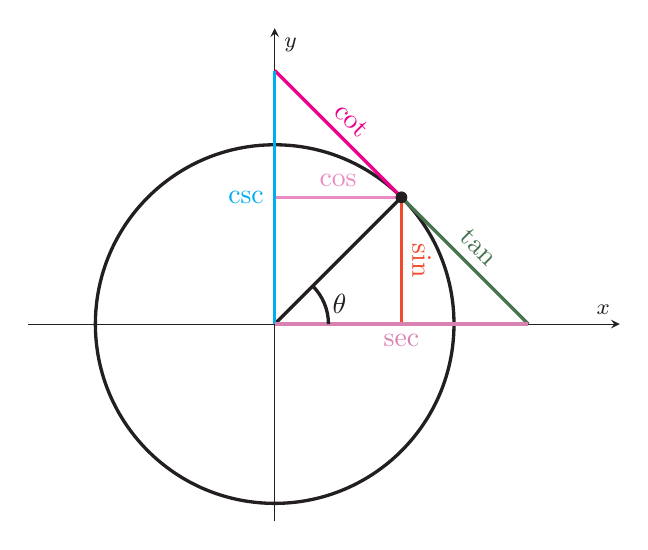
\begin{tikzpicture}
                    \begin{axis}[
                        My Style 1,
                        xmin=-1.1,
                        xmax=1.65,
                        ymin=-1.1,
                        ymax=1.65,
                        width=0.75\linewidth
                    ]
                        \draw[black, very thick] (axis cs:0,0) circle (1);
                        \draw[black, very thick] (axis cs:0,0) -- (45:1);
                        \draw[RedOrange, very thick] (45:1) -- ++(axis direction cs:0, {-sin(45)}) node[sloped, midway, above] {$\sin$};
                        \draw[Violet, very thick] (45:1) -- ++(axis direction cs:{-cos(45)}, 0) node[sloped, midway, above] {$\cos$};
                        \draw[Green, very thick] (45:1) -- ++(axis direction cs:{sec(45)-cos(45)}, {-sin(45)}) node[sloped, midway, above] {$\tan$};
                        \draw[Magenta, very thick] (45:1) -- ++(axis direction cs:{-cos(45)}, {(1/(sin(45)))-sin(45)}) node[sloped, midway, above] {$\cot$};
                        \draw[Cyan, very thick] (axis cs:0,0) -- ++(axis direction cs:0, {1/(sin(45))}) node[midway, left] {$\csc$};
                        \draw[Orchid, very thick] (axis cs:0,0) -- ++(axis direction cs:{sec(45)}, 0) node[sloped, midway, below] {$\sec$};
                        \draw[black, very thick] (axis cs:0.3,0) arc[start angle=0, end angle=45, radius=0.3] node[right, shift={(axis direction cs:0.05,-0.1)}] {$\theta$};
                        \node[shape=circle, fill=black, inner sep=1.5pt] at (45:1) {};
                    \end{axis}
                \end{tikzpicture}
            \end{SummaryBox}
            
            \begin{SummaryBox}[title=Properties of trigonometric functions]
                \begin{itemize}[leftmargin=*]
                    \item $y = \pm a\sin(nt)$
                    \begin{itemize}[topsep=0pt]
                        \item The period of $\frac{2\pi}{n}$.
                        \item The amplitude is $a$.
                        \item The range is $[-a,a]$.
                    \end{itemize}
                    \item $y = \pm a\cos(nt)$
                    \begin{itemize}[topsep=0pt]
                        \item The period of $\frac{2\pi}{n}$.
                        \item The amplitude is $a$.
                        \item The range is $[-a,a]$.
                    \end{itemize}
                    \item $y = a\tan(nt)$
                    \begin{itemize}[topsep=0pt]
                        \item The period of $\frac{\pi}{n}$.
                        \item The vertical asymptotes have equations $t = \frac{(2k + 1)\pi}{2n}$ where $k \in \mathbb{Z}$.
                        \item The axis intercepts are at $t = \frac{k\pi}{n}$ where $k \in \mathbb{Z}$.
                    \end{itemize}
                \end{itemize}
            \end{SummaryBox}
            
            \begin{SummaryBox}[title=Trigonometric identities]
                \begin{SummaryExtensionBox}[title=Pythagorean identities]
                    \begin{multicols}{2}
                        \begin{itemize}[leftmargin=*]
                            \item $\cos^2(x) + \sin^2(x) = 1$
                            \item $\sec^2(x) - \tan^2(x) = 1$
                            \item $\csc^2(x) - \cot^2(x) = 1$
                        \end{itemize}
                    \end{multicols}
                \end{SummaryExtensionBox}
                
                \begin{SummaryExtensionBox}[title=Double-angle identities]
                    \begin{multicols}{2}
                        \begin{itemize}[leftmargin=*]
                            \item $\sin(2x) = 2\sin(x)\cos(x)$
                            \item $\cos(2x) = 2\cos^2(x) - 1$
                            \item $\cos(2x) = 1 - 2\sin^2(x)$
                            \item $\cos(2x) = \cos^2(x) - \sin^2(x)$
                            \item $\tan(2x) = \frac{2\tan(x)}{1-\tan^2(x)}$
                        \end{itemize}
                    \end{multicols}
                \end{SummaryExtensionBox}
                
                \begin{SummaryExtensionBox}[title=Sum/Difference identities]
                    \begin{multicols}{2}
                        \begin{itemize}[leftmargin=*]
                            \item $\sin(s+t) = \sin(s)\cos(t) + \cos(s)\sin(t)$    
                            \item $\sin(s-t) = \sin(s)\cos(t) - \cos(s)\sin(t)$
                            \item $\cos(s+t) = \cos(s)\cos(t) - \sin(s)\sin(t)$
                            \item $\cos(s-t) = \cos(s)\cos(t) + \sin(s)\sin(t)$
                            \item $\tan(s+t) = \frac{\tan(s) + \tan(t)}{1 - \tan(s)\tan(t)}$
                            \item $\tan(s-t) = \frac{\tan(s) - \tan(t)}{1 + \tan(s)\tan(t)}$
                        \end{itemize}
                    \end{multicols}
                \end{SummaryExtensionBox}
                
                \begin{SummaryExtensionBox}[title=Product-to-sum identities]
                    \begin{multicols}{2}
                        \begin{itemize}[leftmargin=*]
                            \item $\cos(s)\cos(t) = \frac{\cos(s-t) + \cos(s+t)}{2}$
                            \item $\sin(s)\sin(t) = \frac{\cos(s-t) - \cos(s+t)}{2}$
                            \item $\sin(s)\cos(t) = \frac{\sin(s+t) + \sin(s-t)}{2}$
                            \item $\cos(s)\sin(t) = \frac{\sin(s+t) - \sin(s-t)}{2}$
                        \end{itemize}
                    \end{multicols}
                \end{SummaryExtensionBox}
                
                \begin{SummaryExtensionBox}[title=Triple-angle identities]
                    \begin{multicols}{2}
                        \begin{itemize}[leftmargin=*]
                            \item $\sin(3x) = -\sin^3(x) + 3\cos^2(x)\sin(x)$
                            \item $\sin(3x) = -4\sin^3(x) + 3\sin(x)$
                            \item $\cos(3x) = \cos^3(x) - 3\sin^2(x)\cos(x)$
                            \item $\cos(3x) = 4\cos^3(x) - 3\cos(x)$
                            \item $\tan(3x) = \frac{3\tan(x) - \tan^3(x)}{1-3\tan^2(x)}$
                            \item $\cot(3x) = \frac{3\cot(x) - \cot^3(x)}{1-3\cot^2(x)}$
                        \end{itemize}
                    \end{multicols}
                \end{SummaryExtensionBox}
            \end{SummaryBox}
            
            \begin{SummaryBox}[title=General solutions]
                \begin{SummaryExtensionBox}[title=General solutions for \texorpdfstring{$\bm{\sin(x)}$}{$\sin(x)$}, list text={General solutions for $\sin(x)$}, ams align* upper]
                    \sin(\theta) &= \alpha, a \in [-1,1] \\
                    \therefore \theta &= 2n\pi + \sin^{-1}(\alpha), n \in \mathbb{Z} \quad \text{or} \\
                                      &= (2n + 1)\pi - \sin^{-1}(\alpha), n \in \mathbb{Z}; \\
                                      &= n\pi + (-1)^n\sin^{-1}(\alpha), n \in \mathbb{Z} \quad \text{(concise)}
                \end{SummaryExtensionBox}
                
                \begin{SummaryExtensionBox}[title=General solutions for \texorpdfstring{$\bm{\cos(x)}$}{$\cos(x)$}, list text={General solutions for $\cos(x)$}, ams align* upper]
                    \cos(\theta) &= \alpha, a \in [-1,1] \\
                    \therefore \theta &= 2n\pi \pm \cos^{-1}(\alpha), n \in \mathbb{Z}
                \end{SummaryExtensionBox}
                
                \begin{SummaryExtensionBox}[title=General solutions for \texorpdfstring{$\bm{\tan(x)}$}{$\tan(x)$}, list text={General solutions for $\tan(x)$}, ams align* upper]
                    \tan(\theta) &= \alpha, a \in [-1,1] \\
                    \therefore \theta &= n\pi + \tan^{-1}(\alpha), n \in \mathbb{Z}
                \end{SummaryExtensionBox}
            \end{SummaryBox}
            
            \begin{SummaryBox}[title=Period of two trigonometric functions' sum/difference, ams align* lower]
                \begin{itemize}[leftmargin=*]
                    \item For two trigonometric functions $f$ and $g$ which are being added to (or subtracted from) each other to produce the function $h$, the period of $h$ is the LCM (lowest common multiple) of the respective periods of $f$ and $g$.
                \end{itemize}
                \tcblower
                \text{Let } f(x)   &= a\sin(bx+c) \\
                \text{Let } g(x)   &= k\cos(mx+n) \\[\belowdisplayskip]
                %
                \text{Let } h(x)   &= f(x) + g(x) \\
                                   &= a\sin(bx+c) + k\cos(mx+n) \\[\belowdisplayskip]
                %
                \per(f)            &= \frac{2\pi}{b} \\
                \per(g)            &= \frac{2\pi}{m} \\
                \therefore \per(h) &= \lcm\pars*{\frac{2\pi}{b}, \frac{2\pi}{m}}
            \end{SummaryBox}
            
            \pagebreak
            
        \section{Differentiation}
            
            \begin{SummaryBox}[title=Average rate of change]
                \begin{itemize}[leftmargin=*]
                    \item For any function $y = f(x)$, the \textbf{average rate of change} of $y$ with respect to $x$ over the interval $[a,b]$ is the gradient of the line through the two points $A(a,f(a))$ and $B(b,f(b))$.
                    \[
                        \text{Average rate of change} = \frac{f(b) - f(a)}{b - a}
                    \]
                \end{itemize}
            \end{SummaryBox}
            
            \begin{SummaryBox}[title=Differentiation from first principles]
                \begin{itemize}[leftmargin=*]
                    \item The \textbf{derivative} of the function $f$ is denoted by $f'$ and is defined by:
                    \[
                        f'(x) = \lim\limits_{h \to 0} \frac{f(x+h) - f(x)}{h}
                    \]
                    \item The derivative of a function $f$ with respect to $x$ when $x=a$ is also known as the \textbf{instantaneous rate of change} of $f$ with respect to $x$ when $x=a$.
                \end{itemize}
            \end{SummaryBox}
            
            \begin{SummaryBox}[title=Derivative rules]
                \begin{SummaryExtensionBox}[title=Differentiation results]
                    \begin{itemize}[leftmargin=*]
                        \item \textbf{Constant function:} $f(x) = c \implies f'(x) = 0$
                        \item \textbf{Multiple:} $f(x) = k \cdot g(x) \implies f'(x) = k \cdot g'(x)$
                        \item \textbf{Sum:} $f(x) = g(x) + h(x) \implies f'(x) = g'(x) + h'(x)$
                        \item \textbf{Difference:} $f(x) = g(x) - h(x) \implies f'(x) = g'(x) - h'(x)$
                    \end{itemize}
                \end{SummaryExtensionBox}
            \end{SummaryBox}

            \begin{SummaryBox}[title=Chain rule]
                When you have a function, \( q(x) \), that can be expressed as the composition of two simpler functions, \( u = g(x) \) and \( q(x) = f(u) \), which are `chained' together: \( x \xrightarrow{g} u \xrightarrow{f} y \), you can use the \textbf{chain rule} to differentiate such a function like so:
                \[
                    q'(x) = f'(g(x)) \cdot g'(x)
                \]
                or, in Leibniz notation, where \( u = g(x) \) and \( y = f(u) \):
                \[
                    \diff[y]{x} = \diff[y]{u} \cdot \diff[u]{x}
                \]
            \end{SummaryBox}
            
            \begin{SummaryBox}[title=Limits]
                \begin{SummaryExtensionBox}[title=Algebra of limits]
                    \begin{itemize}[leftmargin=*]
                        \item \textbf{Sum:} $\lim\limits_{x \to a} \pars*{ f(x) + g(x) } = \lim\limits_{x \to a} \pars*{ f(x) } + \lim\limits_{x \to a} \pars*{ g(x) }$
                        \item \textbf{Multiple:} $\lim\limits_{x \to a} \pars*{ k \cdot f(x) } = k \cdot \lim\limits_{x \to a} \pars*{ f(x) }, k \in \mathbb{R}$
                        \item \textbf{Product:} $\lim\limits_{x \to a} \pars*{ f(x) \cdot g(x) } = \lim\limits_{x \to a} \pars*{ f(x) } \cdot \lim\limits_{x \to a} \pars*{ g(x) }$
                        \item \textbf{Quotient:} $\lim\limits_{x \to a} \pars*{ \frac{f(x)}{g(x)} } = \frac{\lim\limits_{x \to a} \pars*{ f(x) }}{\lim\limits_{x \to a} \pars*{ g(x) }}, \lim\limits_{x \to a} \pars*{ g(x) } \neq 0$
                    \end{itemize}
                \end{SummaryExtensionBox}
                
                \begin{SummaryExtensionBox}[title=Left and right limits]
                    \begin{itemize}[leftmargin=*]
                        \item If the value of $f(x)$ approaches the number $p$ as $x$ approaches $a$ from the right-hand side, the it is written as $\lim\limits_{x \to a^+} f(x) = p$.
                        \item If the value of $f(x)$ approaches the number $p$ as $x$ approaches $a$ from the left-hand side, the it is written as $\lim\limits_{x \to a^-} f(x) = p$.
                        \item For $\lim\limits_{x \to a} f(x)$ to exist, $\lim\limits_{x \to a^+} f(x)$ and $\lim\limits_{x \to a^-} f(x)$ must be equal.
                    \end{itemize}
                \end{SummaryExtensionBox}
            \end{SummaryBox}
            
            \begin{SummaryBox}[title=Continuity of a function]
                \begin{itemize}[leftmargin=*]
                    \item A function $f$ is \textbf{continuous} at the point $x=a$ if the following conditions are met:
                    \begin{itemize}[topsep=0pt]
                        \item $f(a)$ is defined.
                        \item $\lim\limits_{x \to a} f(x) = f(a)$
                    \end{itemize}
                \end{itemize}
            \end{SummaryBox}
            
            \begin{SummaryBox}[title=Differentiability of a function]
                \begin{itemize}[leftmargin=*]
                    \item A function $f$ is said to be differentiable at $x=a$ if $\lim\limits_{h \to 0} \frac{f(a+h) - f(a)}{h}$ exists.
                    \item If a function is differentiable at a point, then it is also continuous at that point (the same cannot be said for the converse statement).
                    \item An easy way to remember this is that a function is \textbf{not differentiable} at a \textit{sharp corner} or a \textit{cusp} (a sharp point where two points meet).
                \end{itemize}
            \end{SummaryBox}
            
            \begin{SummaryBox}[title=Tangent line]
                \begin{itemize}[leftmargin=*]
                    \item The \textbf{tangent line} to the graph of the function $f$ at the point $(a, f(a))$ is defined to be the line through $(a, f(a))$ with the gradient $f'(a)$.
                    \item The equation of the tangent line to the graph of $y = f(x)$ at the point $(a, f(a))$ can be found using the formula:
                    \[
                        y - f(a) = f'(a) \cdot (x - a)
                    \]
                \end{itemize}
            \end{SummaryBox}
            
            \begin{SummaryBox}[title=Normal line]
                \begin{itemize}[leftmargin=*]
                    \item The \textbf{normal line} to the graph of the function $f$ at the point $(a, f(a))$ is defined to be the line through $(a, f(a))$ and is perpendicular to the tangent to the function $f$ at that point.
                    \item The equation of the tangent line to the graph of $y = f(x)$ at the point $(a, f(a))$ can be found using the formula:
                    \[
                        y - f(a) = -\frac{1}{f'(a)} \cdot (x - a)
                    \]
                \end{itemize}
            \end{SummaryBox}
            
            \begin{SummaryBox}[title=Second derivative of a function (concavity), leftlower=0pt, rightlower=0pt]
                \begin{itemize}[leftmargin=*]
                    \item Let $f$ be a function defined on an interval $(a,b)$, and assume that both $f'(x)$ and $f''(x)$ exist for all $x \in (a,b)$.
                    \item If $\forall x \in (a,b): \highmath{$f''(x) > 0$}$, then the gradient of the curve $y=f(x)$ is increasing in the interval $(a,b)$. The curve is \textbf{concave up} (\textit{i.e.,} it has a \textbf{local minimum} in the interval $(a,b)$).
                    \item If $\forall x \in (a,b): \highmath{$f''(x) < 0$}$, then the gradient of the curve $y=f(x)$ is decreasing in the interval $(a,b)$. The curve is \textbf{concave down} (\textit{i.e.,} it has a \textbf{local maximum} in the interval $(a,b)$).
                    \item If \highmath{$f''(x) = 0$} for $x=a$, then there is a \textbf{stationary point of inflection} in the curve $y=f(x)$ at the point when $x=a$.
                \end{itemize}
                \tcblower
                \begin{tblr}{colspec={X[c]|X[c]}}
                    {\begin{tikzpicture}
                        \begin{axis}[
                            My Style 1,
                            xmin=-0.25,
                            xmax=2,
                            ymin=-0.25,
                            ymax=2,
                            extra x ticks={0.2,1.5},
                            extra x tick labels={$a$, $b$}
                        ]
                            \node[black, shift={(-2.5mm,-2.5mm)}, align=center] at (axis cs:0,0) {$O$};
                            \draw[black, thick, {Circle[open]}-{Circle[open]}] (axis cs:0.2,1.2) .. controls (axis cs:0.7,1.1) and (axis cs:1.1,0.4) .. (axis cs:1.5, 1.55);
                            \filldraw[black] (axis cs:0.985,0.8875) circle (3pt);
                        \end{axis}
                    \end{tikzpicture}\\
                    This function is \textbf{concave up} over $\pars*{a, b}$}
                    
                    &
                    
                    {\begin{tikzpicture}
                        \begin{axis}[
                            My Style 1,
                            xmin=-0.25,
                            xmax=2,
                            ymin=-0.25,
                            ymax=2,
                            extra x ticks={0.2,1.5},
                            extra x tick labels={$a$, $b$}
                        ]
                            \node[black, shift={(-2.5mm,-2.5mm)}, align=center] at (axis cs:0,0) {$O$};
                            \draw[black, thick, {Circle[open]}-{Circle[open]}] (axis cs:0.2,0.4) .. controls (axis cs:0.7,1.4) and (axis cs:1.2,0.6) .. (axis cs:1.5,0.4);
                            \filldraw[black] (axis cs:0.725,0.905) circle (3pt);
                        \end{axis}
                    \end{tikzpicture}\\
                    This function is \textbf{concave down} over $\pars*{a, b}$}
                \end{tblr}
            \end{SummaryBox}

            \begin{SummaryBox}[title=Newton's method]
                To approximate solutions to equations of the form \( f(x) = 0 \) for \( x \), we can use Newton's method:
                \[
                    x_{n + 1} = x_n - \frac{f(x_n)}{f'(x_n)}, \quad \text{where } x_{n + 1} \text{ is the next guess}
                \]
                This generates a sequence of \( x \) values where eventually it will converge to a root of the function \( f \).

                Beware, this method may not work as intended if:
                \begin{itemize}[leftmargin=*]
                    \item your initial guess, \( x_0 \), is too close to another root, as it will (likely) converge to that root instead of a ``desired'' root instead;
                    \item the tangent at your initial guess, \( x_n \), is so steep and so is the next guess' tangent in such a way that it leads back to the preivous guess, causing Newton's method to get stuck in an oscillation between \( x_n \) and \( x_{n + 1} \);
                    \item \( x_{n} \), is too close to a stationary point, making the next guess very far away, pushing it further away from the root;
                    \item \( f(x_n) \) or \( f'(x_n) \) does not exist for \( x_n \);
                    \item \( f'(x_n) = 0 \), making the fractional part of the formula undefined.
                \end{itemize}
            \end{SummaryBox}
            
            \pagebreak
            
        \section{Integration}
            
            \begin{SummaryBox}[title=Estimating the area under a graph]
                \begin{SummaryExtensionBox}[title=Left-endpoint estimate, sidebyside, righthand ratio=0.345, leftupper=3mm, leftlower=0pt, rightlower=0pt, center lower]
                    \begin{itemize}[leftmargin=*]
                        \item The formula for the left-endpoint estimate for a function $f$ over the domain $[a,b]$ with rectangles of width $w$ is as follows:
                        \[
                            \text{Area}_{\text{est.}} = \sum\limits^{(b - a)/w}_{k=1} w \cdot f\pars*{a + w \cdot \pars*{k-1}}
                        \]
                        \item For a function $f$ that is\dots
                        \begin{itemize}[topsep=0pt]
                            \item strictly increasing in the domain $[a,b]$, the left-endpoint estimate $\leq$ actual area.
                            \item strictly decreasing in the domain $[a,b]$, the left-endpoint estimate $\geq$ actual area.
                        \end{itemize}
                    \end{itemize}
                    \tcblower
                    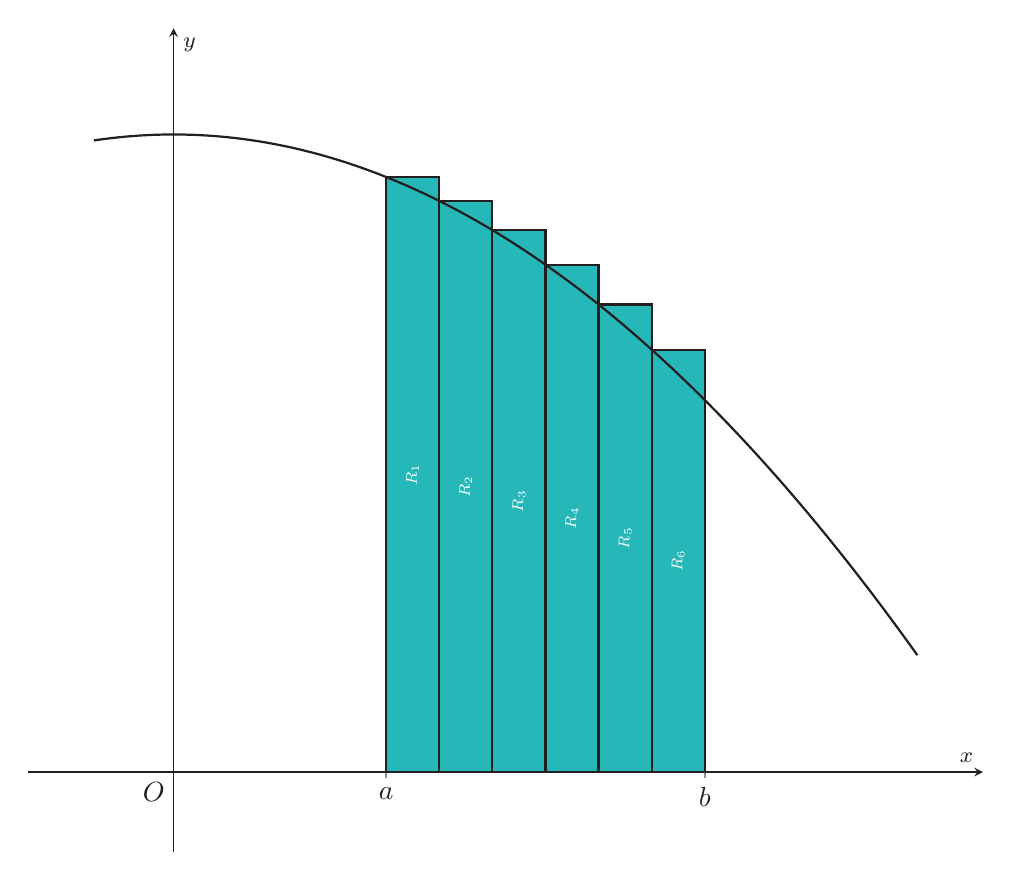
\begin{tikzpicture}
                        \begin{axis}[
                            My Style 1,
                            xmin=-0.75,
                            xmax=7,
                            ymin=-0.75,
                            ymax=7,
                            extra x ticks={2,5},
                            extra x tick labels={$a$, $b$},
                            declare function={f(\x)={ 6 - (0.1 * ((\x)^2)) };},
                            width=\linewidth,
                            scale only axis
                        ]
                            \node[black, shift={(-2.5mm,-2.5mm)}, align=center] at (axis cs:0,0) {$O$};
                            \foreach \x in {1,...,6} {
                                \edef\temp{
                                    \noexpand \draw[thick, black, shaded area] (axis cs:{2+0.5*(\x-1)},0) rectangle (axis cs:{2+0.5*(\x-1)+0.5},{f(2+0.5*(\x-1))}) node[midway, scale=0.8, rotate=90, white] {\noexpand\scriptsize $R_{\x}$};
                                }
                                \temp
                            }
                            \addplot[black, thick, domain=-0.75:7] {f(x)};
                        \end{axis}
                    \end{tikzpicture}
                \end{SummaryExtensionBox}
                
                \begin{SummaryExtensionBox}[title=Right-endpoint estimate, sidebyside, righthand ratio=0.345, leftupper=3mm, leftlower=0pt, rightlower=0pt, center lower]
                    \begin{itemize}[leftmargin=*]
                        \item The formula for the right-endpoint estimate for a function $f$ over the domain $[a,b]$ with rectangles of width $w$ is as follows:
                        \[
                            \text{Area}_{\text{est.}} = \sum\limits^{(b - a)/w}_{k=1} w \cdot f\pars*{a + w k}
                        \]
                        \item For a function $f$ that is\dots
                        \begin{itemize}[topsep=0pt]
                            \item strictly increasing in the domain $[a,b]$, the left-endpoint estimate $\geq$ actual area.
                            \item strictly decreasing in the domain $[a,b]$, the left-endpoint estimate $\leq$ actual area.
                        \end{itemize}
                    \end{itemize}
                    \tcblower
                    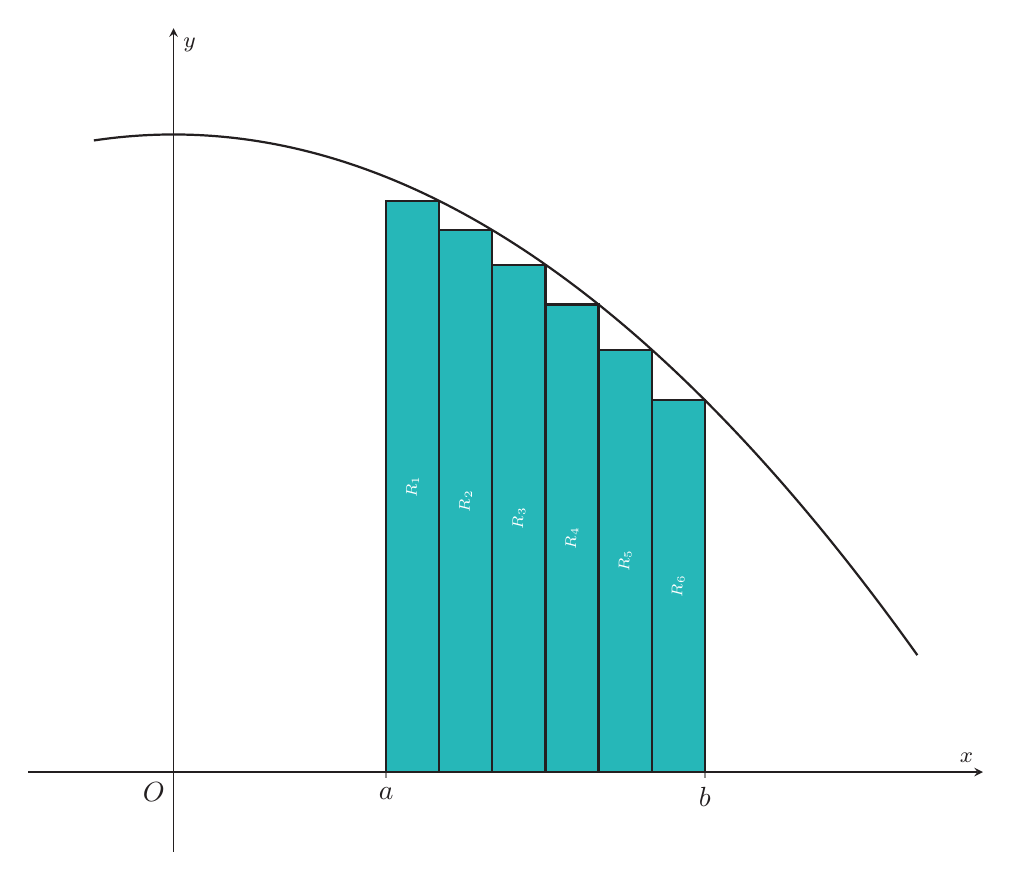
\begin{tikzpicture}
                        \begin{axis}[
                            My Style 1,
                            xmin=-0.75,
                            xmax=7,
                            ymin=-0.75,
                            ymax=7,
                            extra x ticks={2,5},
                            extra x tick labels={$a$, $b$},
                            declare function={f(\x)={ 6 - (0.1 * ((\x)^2)) };},
                            width=\linewidth,
                            scale only axis
                        ]
                            \node[black, shift={(-2.5mm,-2.5mm)}, align=center] at (axis cs:0,0) {$O$};
                            \foreach \x in {1,...,6} {
                                \edef\temp{
                                    \noexpand \draw[thick, black, shaded area] (axis cs:{2+0.5*(\x-1)},0) rectangle (axis cs:{2+0.5*(\x-1)+0.5},{f(2+0.5*\x)}) node[midway, scale=0.8, rotate=90, white] {\noexpand\scriptsize $R_{\x}$};
                                }
                                \temp
                            }
                            \addplot[black, thick, domain=-0.75:7] {f(x)};
                        \end{axis}
                    \end{tikzpicture}
                \end{SummaryExtensionBox}
                
                \begin{SummaryExtensionBox}[title=Trapezium estimate, sidebyside, righthand ratio=0.345, leftupper=3mm, leftlower=0pt, rightlower=0pt, center lower]
                    \begin{itemize}[leftmargin=*]
                        \item The formula for the right-endpoint estimate for a function $f$ over the domain $[a,b]$ with rectangles of width $w$ is as follows:
                    \end{itemize}
                    \[
                        \text{Area}_{\text{est.}} = \sum\limits^{(b - a)/w}_{k=1} w \cdot \bracs*{ f\pars*{a + w \cdot \pars*{k-1}} + f\pars*{a + w k} }
                    \]
                    \tcblower
                    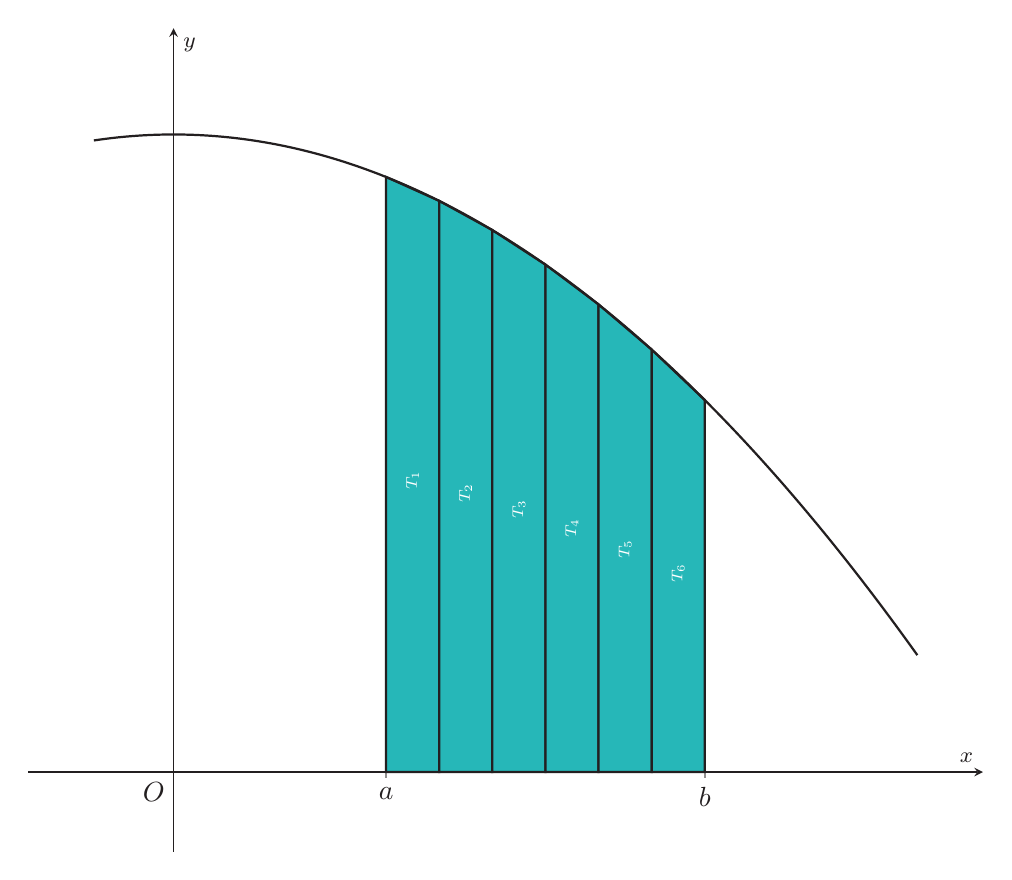
\begin{tikzpicture}
                        \begin{axis}[
                            My Style 1,
                            xmin=-0.75,
                            xmax=7,
                            ymin=-0.75,
                            ymax=7,
                            extra x ticks={2,5},
                            extra x tick labels={$a$, $b$},
                            declare function={f(\x)={ 6 - (0.1 * ((\x)^2)) };},
                            width=\linewidth,
                            scale only axis
                        ]
                            \node[black, shift={(-2.5mm,-2.5mm)}, align=center] at (axis cs:0,0) {$O$};
                            \foreach \x in {1,...,6} {
                                \edef\temp{
                                    \noexpand\draw[thick, black, shaded area] (axis cs:{2+0.5*(\x-1)}, 0) -- (axis cs:{2+0.5*(\x-1)}, {f(2+0.5*(\x-1))}) -- (axis cs:{2+0.5*(\x-1)+0.5}, {f(2+0.5*\x)}) -- (axis cs:{2+0.5*(\x-1)+0.5}, 0) -- cycle;
                                    \noexpand\node[scale=0.8, rotate=90, white] at (axis cs:{{2+0.5*(\x-1)+0.25}}, {f(2+0.5*(\x-1)+0.25)/2}) {\noexpand\scriptsize $T_{\x}$};
                                }
                                \temp
                            }
                            \addplot[black, thick, domain=-0.75:7] {f(x)};
                        \end{axis}
                    \end{tikzpicture}
                \end{SummaryExtensionBox}
            \end{SummaryBox}
            
            \begin{SummaryBox}[title=The fundamental theorem of calculus]
                \[
                    \diff{x}\bracs*{F(x)} = f(x) \quad \implies \quad \int\limits^{b}_{a} f(x)\intd{x} = \bracs*{F(x)}^{b}_{a} = F(b) - F(a)
                \]
                \begin{itemize}[leftmargin=*, topsep=0pt]
                    \item As the constant $(+C)$ cancels out, we normally ignore it and take the antiderivative of $f$ with $C=0$.
                \end{itemize}
            \end{SummaryBox}
            
            \begin{SummaryBox}[title=Antidifferentiation rules]
                \begin{SummaryExtensionBox}[title=Antidifferentiation results]
                    \begin{itemize}[leftmargin=*]
                        \item \textbf{Sum:} $\int \bracs*{f(x) + g(x)}\intd{x} = \int f(x)\intd{x} + \int g(x)\intd{x}$
                        \item \textbf{Difference:} $\int \bracs*{f(x) - g(x)}\intd{x} = \int f(x)\intd{x} - \int g(x)\intd{x}$
                        \item \textbf{Multiple:} $\int \bracs*{k \cdot f(x)}\intd{x} = k \cdot \int f(x)\intd{x}, k \in \mathbb{R}$
                    \end{itemize}
                \end{SummaryExtensionBox}
                
                \begin{SummaryExtensionBox}[title=Properties of the definite integral]
                    \begin{itemize}[leftmargin=*]
                        \item $\int\limits_a^b f(x)\intd{x} = \int\limits_a^c f(x)\intd{x} + \int\limits_c^b f(x)\intd{x}$
                        \item $\int\limits_a^a f(x)\intd{x} = 0$
                        \item $\int\limits_a^b \bracs*{k \cdot f(x)}\intd{x} = k \cdot \int\limits_a^b f(x)\intd{x}$
                        \item $\int\limits_a^b \bracs*{f(x) \pm g(x)}\intd{x} = \int\limits_a^b f(x)\intd{x} \pm \int\limits_a^b g(x)\intd{x}$
                        \item $\int\limits_a^b f(x)\intd{x} = -\int\limits_b^a f(x)\intd{x}$
                    \end{itemize}
                \end{SummaryExtensionBox}
            \end{SummaryBox}
            
            \begin{SummaryBox}[title=Signed area]
                \begin{itemize}[leftmargin=*]
                    \item For any continuous function $f$ on an interval $[a,b]$, the \textbf{definite integral} $\int\limits^{b}_{a} f(x)\intd{x}$ gives the \textbf{signed area} enclosed by the graph of $y=f(x)$ between $x=a$ and $x=b$.
                    \item To get the \textbf{unsigned area}, just take the absolute value of the function like so: $\int\limits^{b}_{a} \verts*{f(x)}\intd{x}$.
                \end{itemize}
            \end{SummaryBox}
            
            \begin{SummaryBox}[title=Average value of a function, sidebyside, righthand ratio=0.45, leftlower=0pt, rightlower=0pt, center lower]
                \begin{itemize}[leftmargin=*]
                    \item The \textbf{average value} of a continuous function $f$ over an interval $[a,b]$ is:
                    \[
                        \frac{1}{b-a} \cdot \int\limits_{a}^{b} f(x)\intd{x}
                    \]
                    \item In terms of the graph of $y=f(x)$, the average value is the \textbf{height of a rectangle} having the same area as the area under the graph for the interval $[a,b]$ (the interval forms the rectangle's base).
                \end{itemize}
                \tcblower
                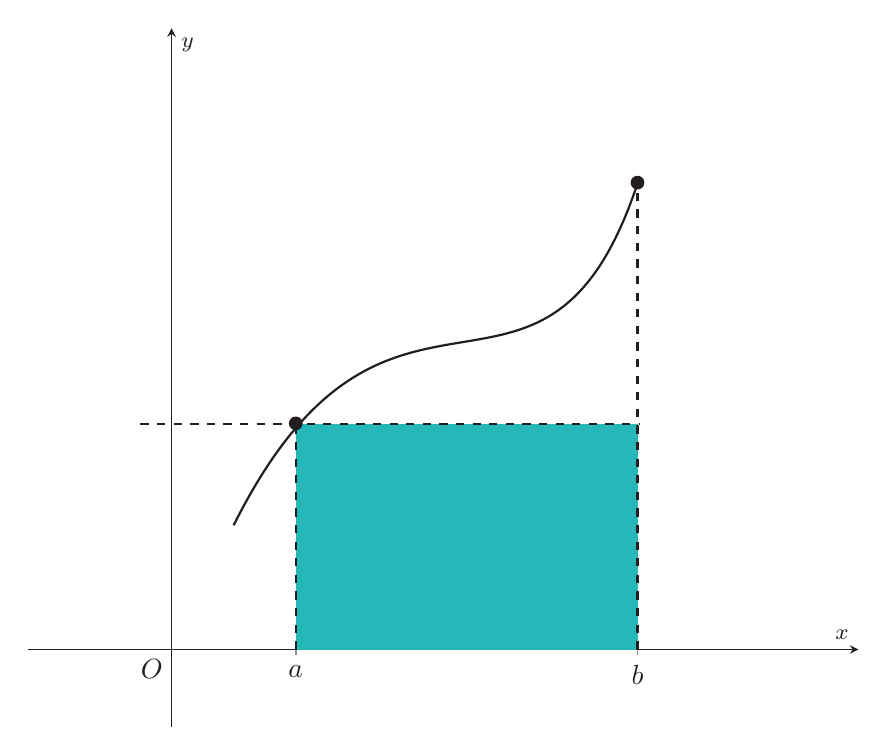
\begin{tikzpicture}
                    \begin{axis}[
                        My Style 1,
                        xmin=-0.25,
                        xmax=2,
                        ymin=-0.25,
                        ymax=2,
                        extra x ticks={0.4,1.5},
                        extra x tick labels={$a$, $b$},
                        width=\linewidth
                    ]
                        \node[black, shift={(-2.5mm,-2.5mm)}, align=center] at (axis cs:0,0) {$O$};
                        \draw[black, thick] (axis cs:0.2,0.4) .. controls (axis cs:0.7,1.4) and (axis cs:1.2,0.6) .. (axis cs:1.5,1.5);
                        \path[thick, dashed, black, shaded area] (axis cs:0.4,0) -- ++(axis direction cs:0,0.725) -- ++(axis direction cs:1.5-0.4,0) -- ++(axis direction cs:0,-0.725);
                        \draw[black, thick, dashed, -{Circle}] (axis cs:0.4,0) -- ++(axis direction cs:0,0.75);
                        \draw[black, thick, dashed, -{Circle}] (axis cs:1.5,0) -- ++(axis direction cs:0,1.525);
                        \draw[black, thick, dashed] (axis cs:-0.1,0.725) -- ++(axis direction cs:1.6075,0);
                    \end{axis}
                \end{tikzpicture}
            \end{SummaryBox}
            
            \pagebreak
            
        \section{Probability}
            
            \begin{SummaryBox}[title=Basic laws of probability]
                \begin{itemize}[leftmargin=*]
                    \item \textbf{Total law of probability:} $\forall x \subseteq \mathcal{E}:\Pr(X=x) = 1$
                    \item $\Pr(X=x) \geq 0 \iff x \in \mathcal{E}$
                    \item \textbf{Addition rule:} $\Pr(A \cup B) = \Pr(A) + \Pr(B) - \Pr(A \cap B)$
                    \item $\Pr(\varnothing) = 0$
                    \item $\Pr(A') = 1 - A$, where $A'$ is the complement of $A$.
                \end{itemize}
            \end{SummaryBox}
            
            \begin{SummaryBox}[title=Mutually exclusive events]
                \begin{itemize}[leftmargin=*]
                    \item Two events $A$ and $B$ are mutually exclusive if:
                    \[
                        \Pr(A \cap B) = 0
                    \]
                    \item For mutually exclusive events, the addition rules becomes:
                    \[
                        \Pr(A \cup B) = \Pr(A) + \Pr(B)
                    \]
                \end{itemize}
            \end{SummaryBox}
            
            \begin{SummaryBox}[title=Probabilities from data]
                \begin{itemize}[leftmargin=*]
                    \item When the number of trials is sufficiently large, the observed relative frequency of an event $A$ becomes close to the probability $\Pr(A)$. That is,
                    \[
                        \Pr(A) \approx \frac{\text{number of times }A\text{  occurs}}{\text{number of trials}} \quad \text{for a large number of trials}
                    \]
                \end{itemize}
            \end{SummaryBox}
            
            \begin{SummaryBox}[title=Probability tables (Karnaugh maps), center upper, left=0pt, right=0pt]
                \begin{tblr}{colspec={X[c,0.15,mode=dmath] | X[c,0.3,mode=dmath] | X[c,0.3,mode=dmath] | X[c,0.15,mode=dmath]}, cell{1}{2-3}={cmd={\bm}}, cell{2-3}{1}={cmd={\bm}}, cell{2-4}{4}={cmd={\bm}}, cell{4}{2-4}={cmd={\bm}}, hline{2-Y}}
                    \cline{2-3}
                         &    B                &    B'                &              \\
                    A    &    \Pr(A \cap B)    &    \Pr(A \cap B')    &    \Pr(A)    \\
                    A'   &    \Pr(A' \cap B)   &    \Pr(A' \cap B')   &    \Pr(A')   \\
                         &    \Pr(B)           &    \Pr(B')           &    1         \\
                    \cline{2-4}
                \end{tblr}
            \end{SummaryBox}
            
            \begin{SummaryBox}[title=Conditional probability]
                \begin{itemize}[leftmargin=*]
                    \item The \textbf{conditional probability} of an event $A$, given that event $B$ has already occured, is given by:
                    \[
                        \Pr(A \mid B) = \frac{\Pr(A \cap B)}{\Pr(B)} \quad \text{if }\Pr(B) \neq 0
                    \]
                    \item This formula may be rearranged to give the \textbf{multiplication rule of probability:}
                    \[
                        \Pr(A \cap B) = \Pr(A \mid B) \cdot \Pr(B)
                    \]
                \end{itemize}
            \end{SummaryBox}
            
            \begin{SummaryBox}[title=Law of total probability]
                \begin{itemize}[leftmargin=*]
                    \item The \textbf{law of total probability} states that, in the case of two events $A$ and $B$,
                    \[
                        \Pr(A) = \Pr(A \mid B) \cdot \Pr(B) + \Pr(A \mid B') \cdot \Pr(B')
                    \]
                \end{itemize}
            \end{SummaryBox}
            
            \begin{SummaryBox}[title=Independent events]
                \begin{itemize}[leftmargin=*]
                    \item For events $A$ and $B$ with $\Pr(A) \neq 0$ and $\Pr(A) \neq 0$, the following three conditions are all \textbf{equivalent conditions} for the independence of $A$ and $B$:
                    \begin{itemize}[topsep=0pt]
                        \item $\Pr(A \mid B) = \Pr(A)$
                        \item $\Pr(B \mid A) = \Pr(B)$
                        \item $\Pr(A \cap B) = \Pr(A) \cdot \Pr(B)$
                    \end{itemize}
                    \item In the special case that $\Pr(A) = 0$ or $\Pr(B) = 0$, the third condition $( \Pr(A \cap B) = \Pr(A) \cdot \Pr(B) )$ still holds since both sides are zero, so events $A$ and $B$ are still independent.
                \end{itemize}
            \end{SummaryBox}
            
            \begin{SummaryBox}[title=Discrete probability functions]
                \begin{itemize}[leftmargin=*]
                    \item The probability distribution of $X$ is a function $p(x) = Pr(X = x)$ that assigns a probability to each value of $X$. It can be represented by a rule, a table or a graph, and must give a probability $p(x)$ for every value $x$ that $X$ can take.
                    \item For \textit{any} discrete probability function $p(x)$, the following two conditions must hold:
                    \begin{itemize}[topsep=0pt]
                        \item Each value of $p(x)$ belongs to the interval $[0,1]$. That is,
                        \[
                            \forall x \in \dom(p): 0 \leq p(x) \leq 1
                        \]
                        \item The sum of all the values of $p(x)$ must be $1$. That is,
                        \[
                            \sum\limits_{x} p(x) = 1
                        \]
                    \end{itemize}
                    \item The sum of the values of values of $p(x)$ for $x$ between $a$ and $b$ inclusive is written as
                    \[
                        \sum\limits_{a \leq x \leq b} p(x) = \Pr(a \leq X \leq b)
                    \]
                \end{itemize}
            \end{SummaryBox}
            
            \begin{SummaryBox}[title=Population parameters, breakable]
                \begin{SummaryExtensionBox}[title=Expected value]
                    \begin{itemize}[leftmargin=*]
                        \item The \textbf{expected value} of a discrete random variable $X$ is determined by summing the products of each value of $X$ and the probability that $X$ takes that value. That is,
                        \begin{align*}
                            \E(X) &= \sum\limits_x \bracs*{ x \cdot \Pr(X = x) } \\
                                  &= \sum\limits_x \bracs*{ x \cdot p(x) }
                        \end{align*}
                        \item The expected value $\E(X)$ may be considered as the long-run average value of $X$.
                        \item It is generally denoted by $\mu$, and is also called the \textbf{mean} of $X$.
                        \item $\E\bracs*{g(X)} = \sum\limits_x \bracs*{ g(x) \cdot p(x) }$
                        \item $\E(aX + b) = a \cdot \E(X) + b$ \quad (for $a,b$ constant)
                        \begin{itemize}[topsep=0pt]
                            \item Generally, $\E\bracs*{ g(X) } \neq g\bracs*{ \E(X) }$, but the linear case is an exception.
                        \end{itemize}
                        \item If $X$ and $Y$ are two random variables, then $\E(X+Y) = \E(X) + \E(Y)$
                    \end{itemize}
                \end{SummaryExtensionBox}
                
                \begin{SummaryExtensionBox}[title=Variance]
                    \begin{itemize}[leftmargin=*]
                        \item The \textbf{variance} of a random variable $X$ is the measure of the spread of the probability distribution about its mean or expected value $\mu$.
                        \item It is defined as:
                        \begin{align*}
                            \Var(X) &= \E\bracs*{ (X - \mu)^2 } \\
                                    &= \sum\limits_x \bracs*{ (x-\mu)^2 \cdot \Pr(X=x) } \\
                                    &= \sum\limits_x \bracs*{ (x-\mu)^2 \cdot p(x) }
                        \end{align*}
                        \item Alternatively, the computational formula for calculating variance is as such:
                        \[
                            \Var(X) = \E\pars*{X^2} - \bracs*{ \E(X) }^2
                        \]
                        \item It may be considered the long-run average value of the square of the distance from $X$ to $mu$.
                        \item The variance is denoted using $\sigma^2$.
                        \item $\Var(aX + b) = a^2 \cdot \Var(X)$ \quad (for $a,b$ constant)
                    \end{itemize}
                \end{SummaryExtensionBox}
                
                \begin{SummaryExtensionBox}[title=Standard deviation]
                    \begin{itemize}[leftmargin=*]
                        \item The \textbf{standard deviation} is defined as the square-root of the variance $\sigma^2$. That is,
                        \[
                            \sd(X) = \sqrt{\Var(X)}
                        \]
                        \item It is usually denoted with $\sigma$.
                    \end{itemize}
                \end{SummaryExtensionBox}
            \end{SummaryBox}
            
            \begin{SummaryBox}[title=Bernoulli sequence]
                \begin{itemize}[leftmargin=*]
                    \item A \textbf{Bernoulli sequence} is the name used to describe a sequence of repeated trials with the following properties:
                    \begin{itemize}[topsep=0pt]
                        \item Each trial results in one of two outcomes, which are usually designated as either a success, $S$, or a failure, $F$.
                        \item The probability of success on a single trial, $p$, is constant for all trials (and thus the probability of failure on a single trial is $1 - p$).
                        \item The trials are independent (so that the outcome of any trial is not affected by the outcome of any previous trial).
                    \end{itemize}
                \end{itemize}
            \end{SummaryBox}
            
            \begin{SummaryBox}[title=Binomial probability distribution]
                \begin{itemize}[leftmargin=*]
                    \item The number of successes in a Bernoulli sequence of $n$ trials is called a \textbf{binomial random variable} and is said to have a \textbf{binomial probability distribution}.
                    \item If the random variable $X$ is the number of successes in $n$ independent trials, each with probability of success $p$, then $X$ has a \textbf{binomial distribution}, written $X \sim \Bi(n,p)$ and the rule is
                    \[
                        \Pr(X=x) = \binom{n}{x} \cdot p^x \cdot (1-p)^{n-x} \quad x=0,1,\dots,n
                    \]
                    where $\binom{n}{x} = \frac{n!}{x! \cdot (n - x)!}$
                    \item As the value of $p$ increases, the graph of the binomial distribution is more skewed to the right (negatively skewed). A value of $p=0.5$ makes the peak of the graph of $y=p(x)$ line up with the midway of the interval $[0,n]$ of the $x$-axis.
                    
                    \begin{SummaryExtensionBox}[title=Population parameters for the binomial distribution]
                        \begin{itemize}[leftmargin=*]
                            \item $\E(X) = np$
                            \item $\Var(X) = np(1-p)$
                        \end{itemize}
                    \end{SummaryExtensionBox}
                \end{itemize}
            \end{SummaryBox}
            
            \begin{SummaryBox}[title=Probability density functions]
                \begin{itemize}[leftmargin=*]
                    \item In general, the probability density function $f$ is a function with domain some interval (\textit{e.g.,} domain $[c,d]$ or $\mathbb{R}$) such that:
                    \begin{enumerate}[topsep=0pt]
                        \item $\forall x \in \dom(f): f(x) \geq 0$
                        \item The area under the graph of $y=f(x)$ is equal to $1$.
                        \begin{itemize}[topsep=0pt]
                            \item If the domain of $f$ is $[c,d]$, then this condition corresponds to $\int\limits_c^d f(x)\intd{x} = 1$.
                        \end{itemize}
                    \end{enumerate}
                    \item The values of a probability density function $f$ are not probabilities, and $f(x)$ may take values greater than $1$.
                    \item The probability of any specific value of $X$ is $0$. That is, $\Pr(X=a)=0$.
                    \item It follows that all of the following expressions have the same numerical value:
                    \begin{multicols}{4}
                        \begin{itemize}[topsep=0pt]
                            \item $\Pr(a < X < b)$
                            \item $\Pr(a \leq X < b)$
                            \item $\Pr(a < X \leq b)$
                            \item $\Pr(a \leq X \leq b)$
                        \end{itemize}
                    \end{multicols}
                    \item If $f$ has the domain $[c,d]$ and $a \in [c,d]$, then $\Pr(X < a) = \Pr(X \leq a) = \int\limits_c^a f(x)\intd{x}$.
                \end{itemize}
                
                \begin{SummaryExtensionBox}[title=Visualising a probability density function, sidebyside, leftlower=0pt, rightlower=0pt]
                    \begin{itemize}[leftmargin=*]
                        \item If $X$ is a continuous random variable with density function $f$, then
                        \[
                            \Pr(a < X < b) = \int\limits_a^b f(x)\intd{x}
                        \]
                        which is the area of the shaded region.
                    \end{itemize}
                    \tcblower
                    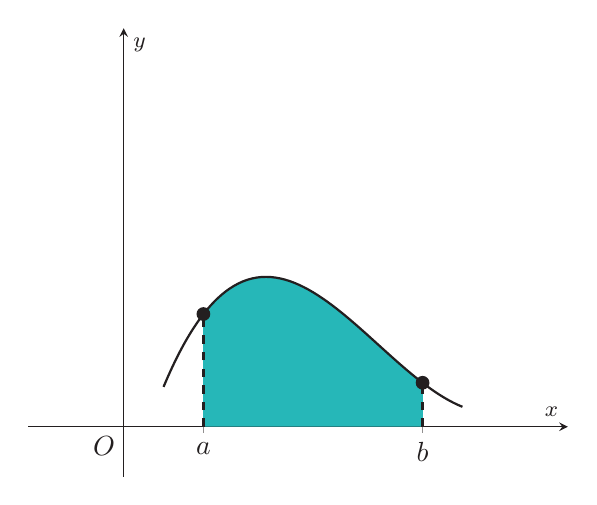
\begin{tikzpicture}
                        \begin{axis}[
                            My Style 1,
                            xmin=-0.25,
                            xmax=2,
                            ymin=-0.25,
                            ymax=2,
                            extra x ticks={0.4,1.5},
                            extra x tick labels={$a$, $b$}
                        ]
                            \node[black, shift={(-2.5mm,-2.5mm)}, align=center] at (axis cs:0,0) {$O$};
                            
                            \begin{scope}
                                \clip[] (axis cs:0.2,0.2) .. controls (axis cs:0.7,1.4) and (axis cs:1.2,0.3) .. (axis cs:1.7,0.1) -- (axis cs:1.7,0) -- (axis cs:0.2,0) -- cycle;
                                \path[black, shaded area] (axis cs:0.4,0) rectangle (axis cs:1.5,1);
                            \end{scope}
                            
                            \draw[black, thick, dashed, -{Circle}] (axis cs:0.4,0) -- (axis cs:0.4,0.6);
                            \draw[black, thick, dashed, -{Circle}] (axis cs:1.5,0) -- (axis cs:1.5,0.255);
                            \draw[black, thick] (axis cs:0.2,0.2) .. controls (axis cs:0.7,1.4) and (axis cs:1.2,0.3) .. (axis cs:1.7,0.1);
                        \end{axis}
                    \end{tikzpicture}
                \end{SummaryExtensionBox}
            \end{SummaryBox}
            
            \begin{SummaryBox}[title=Computing improper integrals]
                \begin{itemize}[leftmargin=*]
                    \item If $\dom(f) = (-\infty,a]$, then $\int\limits_{-\infty}^a f(x)\intd{x} = 1$. This integral is computed as
                    \[
                        \lim\limits_{k \to \infty} \int\limits_{-k}^a f(x)\intd{x}
                    \]
                    \item If $\dom(f) = [a,\infty)$, then $\int\limits_a^\infty f(x)\intd{x} = 1$. This integral is computed as
                    \[
                        \lim\limits_{k \to \infty} \int\limits_a^k f(x)\intd{x}
                    \]
                    \item If $\dom(f) = (-\infty,\infty)$, then $\int\limits_{-\infty}^\infty f(x)\intd{x} = 1$. This integral is computed as
                    \[
                        \lim\limits_{k \to \infty} \int\limits_{-k}^k f(x)\intd{x}
                    \]
                \end{itemize}
            \end{SummaryBox}
            
            \begin{SummaryBox}[title=Properties for a continuous probability distribution, breakable]
                \begin{SummaryExtensionBox}[title=Expected value/mean]
                    \begin{itemize}[leftmargin=*]
                        \item For a continuous random variable $X$ with probability density function $f$, the \textbf{mean} or \textbf{expected value} of $X$ is given by
                        \[
                            \E(X) = \int\limits_{-\infty}^\infty f(x)\intd{x}
                        \]
                        provided the integral exists.
                        \item If $f(x) = 0$ for all $x \notin [c,d]$, then
                        \[
                            \E(X) = \int\limits_c^d f(x)\intd{x}
                        \]
                        \item This definition is consistent with the definition provided in the ``Expected Value'' section of the ``Population parameters'' box. Where appropriate, substitute an integral for the summation symbol and $f$ in place of $p$.
                    \end{itemize}
                \end{SummaryExtensionBox}
                
                \begin{SummaryExtensionBox}[title=Percentiles]
                    \begin{itemize}[leftmargin=*]
                        \item The value $p$ of $X$ which is the solution of an equation of the form
                        \[
                            \int\limits_{-\infty}^p f(x)\intd{x} = q
                        \]
                        is called a \textbf{percentile} of the distribution.
                        \item For example, the 75\textsuperscript{th} percentile is the value $p$ found by taking $q = 75\% = 0.75$.
                    \end{itemize}
                \end{SummaryExtensionBox}
                
                \begin{SummaryExtensionBox}[title=The median]
                    \begin{itemize}[leftmargin=*]
                        \item The \textbf{median} is another measure of centre for a continuous probability distribution.
                        \item The median, $m$, of a continuous random variable $X$ is the value of $X$ such that
                        \[
                            \int\limits_{-\infty}^m f(x)\intd{x} = 0.5
                        \]
                        \item It is also known as the \textbf{50\textsuperscript{th}} percentile.
                    \end{itemize}
                \end{SummaryExtensionBox}
                
                \begin{SummaryExtensionBox}[title=Interquartile range]
                    \begin{itemize}[leftmargin=*]
                        \item The \textbf{interquartile range} is the range of the middle $50\%$ of the distribution; it is the difference between the 75\textsuperscript{th} percentile (also known as Q3) and the 25\textsuperscript{th} percentile (also known as Q1).
                        \[
                            \operatorname{IQR} = b - a
                        \]
                        where $a$ and $b$ are such that
                        \[
                            \int\limits_{-\infty}^a f(x)\intd(x) = 0.25 \quad \text{and} \quad \int\limits_{-\infty}^b f(x)\intd(x) = 0.75
                        \]
                    \end{itemize}
                \end{SummaryExtensionBox}
                
                \begin{SummaryExtensionBox}[title=The variance of a continuous probability distribution, ams align* upper]
                    \Var(X) &= \E\pars*{X^2} - \mu^2 \\
                            &= \E\bracs*{ (X - \mu)^2 } \\
                            &= \int\limits_{-\infty}^\infty \bracs*{ (x-\mu)^2 \cdot f(x) }\intd{x}
                \end{SummaryExtensionBox}
                
                \begin{SummaryExtensionBox}[title=The standard deviation of a continuous probability distribution, ams align* upper]
                    \sd(X) &= \sqrt{ \Var(X) }
                \end{SummaryExtensionBox}
            \end{SummaryBox}
            
            \begin{SummaryBox}[title=The probability density function of \texorpdfstring{$\bm{aX+b}$}{$aX+b$}, list text=The probability density function of $aX+b$]
                \begin{itemize}[leftmargin=*]
                    \item If the probability density function of $X$ has the rule $f(x)$, then the probability density function of $aX + b$ is $\frac{1}{a} \cdot f\pars*{ \frac{x-b}{a} }$ and is described by the transformation
                    \[
                        (x,y) \to \pars*{ ax+b, \frac{y}{a} }
                    \]
                \end{itemize}
            \end{SummaryBox}
            
            \begin{SummaryBox}[title=The standard normal distribution, breakable]
                \begin{itemize}[leftmargin=*]
                    \item A random variable $Z$ with the standard normal distribution has probability density function
                    \[
                        f(x) = \frac{1}{\sqrt{ 2\pi }} \cdot e^{ -\frac{1}{2} \cdot x^2 }
                    \]
                    \item The standard normal distribution has mean $\mu = 0$ and standard deviation $\sigma = 1$.
                \end{itemize}
                
                \begin{SummaryExtensionBox}[title=Transformations of normal distributions]
                    \begin{itemize}[leftmargin=*]
                        \item If $X$ is a \textbf{normally distributed random variable} with mean $\mu$ and standard deviation $\sigma$, then the probability density function of $X$ is given by
                        \[
                            f(x) = \frac{1}{\sigma \cdot \sqrt{ 2\pi }} \cdot e^{ -\frac{1}{2} \cdot \pars*{ \frac{x - \mu}{\sigma} }^2 }
                        \]
                        and
                        \[
                            \Pr(X \leq a) = \Pr\pars*{Z \leq \frac{a - \mu}{\sigma}}
                        \]
                        where $Z$ is the random variable of the standard normal distribution.
                        \begin{itemize}[topsep=0pt]
                            \item The transformation which maps the graph of a normal distribution with mean $\mu$ and standard deviation $\sigma$ to the graph of the standard normal distribution is as follows:
                            \[
                                (x,y) \to \pars*{ \frac{x - \mu}{\sigma}, \sigma y }
                            \]
                            \item Conversely, the transformation which maps the graph of the standard normal distribution to the graph of a normal distribution with mean $\mu$ and standard deviation $\sigma$ is as follows:
                            \[
                                (x,y) \to \pars*{ \sigma x + \mu, \frac{y}{\sigma} }
                            \]
                            \item These transformations are ``area preserving''.
                        \end{itemize}
                    \end{itemize}
                \end{SummaryExtensionBox}
                
                \begin{SummaryExtensionBox}[title=Symmetry properties of the standard normal distribution]
                    \begin{itemize}[leftmargin=*]
                        \item $\Pr(Z > a) = 1 - \Pr(Z \leq a)$
                        \item $\Pr(Z < -a) = \Pr(Z > a)$
                        \item $\begin{aligned}[t] \Pr(-a < Z < a) &= 1 - 2\Pr(Z \geq a) \\ &= 1 - 2\Pr(Z \leq -a) \end{aligned}$
                    \end{itemize}
                \end{SummaryExtensionBox}
            \end{SummaryBox}
            
            \begin{SummaryBox}[title=Empirical formulas, leftlower=0pt, rightlower=0pt, center lower]
                \begin{itemize}[leftmargin=*]
                    \item For a normally distributed random variable, approximately:
                    \begin{itemize}[topsep=0pt]
                        \item $68\%$ of values lie within one standard deviation of the mean, which is the interval $[\mu - \sigma, \mu + \sigma]$.
                        \item $95\%$ of values lie within two standard deviation of the mean, which is the interval $[\mu - 2\sigma, \mu + 2\sigma]$.
                        \item $99.7\%$ of values lie within three standard deviation of the mean, which is the interval $[\mu - 3\sigma, \mu + 3\sigma]$.
                    \end{itemize}
                \end{itemize}
                \tcblower
                \begin{tikzpicture}
                    \begin{axis}[%
                        no markers,
                        domain=0:10,
                        samples=150,
                        axis lines*=left,
                        xlabel=Standard deviations,
                        ylabel=Frequency,
                        height=6cm,
                        width=10cm,
                        xtick={-3, -2, -1, 0, 1, 2, 3},
                        xticklabels={%
                            {$-3$\\$-3\sigma$},
                            {$-2$\\$-2\sigma$},
                            {$-1$\\$-\sigma$},
                            {$0$\\$\mu$},
                            {$1$\\$\sigma$},
                            {$2$\\$2\sigma$},
                            {$3$\\$3\sigma$}
                        },
                        xticklabel style={align=center},
                        label style={font=\footnotesize},
                        major tick style={semithick},
                        ytick=\empty,
                        enlargelimits=false,
                        clip=false,
                        axis on top,
                        grid = major,
                        width=\linewidth
                    ]
                        \addplot [fill=cyan!20, draw=none, domain=-3:3] {gauss(0,1)} \closedcycle;
                        \addplot [fill=Bittersweet!20, draw=none, domain=-3:-2] {gauss(0,1)} \closedcycle;
                        \addplot [fill=Bittersweet!20, draw=none, domain=2:3] {gauss(0,1)} \closedcycle;
                        \addplot [fill=blue!20, draw=none, domain=-2:-1] {gauss(0,1)} \closedcycle;
                        \addplot [fill=blue!20, draw=none, domain=1:2] {gauss(0,1)} \closedcycle;
                        
                        \addplot[] coordinates {(-1,0.4) (1,0.4)};
                        \addplot[] coordinates {(-2,0.3) (2,0.3)};
                        \addplot[] coordinates {(-3,0.2) (3,0.2)};
                        
                        \coordinate (A) at (axis cs: 0, 0.4);
                        \coordinate (B) at (axis cs: 0, 0.3);
                        \coordinate (C) at (axis cs: 0, 0.2);
                        \coordinate (D) at (axis cs: -0.5, 0);
                        \coordinate (E) at (axis cs: 0.5, 0);
                        \coordinate (F) at (axis cs: 1.5, 0);
                        \coordinate (G) at (axis cs: -1.5, 0);
                        \coordinate (H) at (axis cs: 2.5, 0);
                        \coordinate (I) at (axis cs: -2.5, 0);
                    \end{axis}
                    
                    \node[coordinate, pin={68.2\%}] at (A)  {};
                    \node[coordinate, pin={95\%}]   at (B)  {};
                    \node[coordinate, pin={99.7\%}] at (C)  {};
                    \node[coordinate, pin={34.1\%}] at (D)  {};
                    \node[coordinate, pin={34.1\%}] at (E)  {};
                    \node[coordinate, pin={13.6\%}] at (F)  {};
                    \node[coordinate, pin={13.6\%}] at (G)  {};
                    \node[coordinate, pin={2.1\%}]  at (H)  {};
                    \node[coordinate, pin={2.1\%}]  at (I)  {};
                \end{tikzpicture}
            \end{SummaryBox}
            
            \begin{SummaryBox}[title=Normal approximation of a binomial distribution]
                \begin{itemize}[leftmargin=*]
                    \item If $n$ is sufficiently large, the binomial random variable $X$ will be approximately normally distributed, with a mean of $\mu = np$ and a standard deviation of $\sigma = \sqrt{np(1-p)}$.
                    \item One rule of thumb is that $np > 5$ \textbf{and} $n(1-p) > 5$ for a satisfactory approximation.
                \end{itemize}
            \end{SummaryBox}
            
            \pagebreak
            
        \section{Sampling}
            
            \begin{SummaryBox}[title=Sample]
                \begin{itemize}[leftmargin=*]
                    \item A sample of size $n$ is called a \textbf{simple random sample} if it is selected from the population in such a way that every subset of size $n$ has an equal chance of being chosen as the sample.
                    \item In particular, every member of the population must have an equal chance of being included in the sample.
                \end{itemize}
            \end{SummaryBox}
            
            \begin{SummaryBox}[title=Population and sample proportions]
                \begin{itemize}[leftmargin=*]
                    \item The \textbf{population proportion} $p$ is a \textbf{population parameter}; its value is constant. This is also what is used as the value for the probability of success when calculating $\hat{p}$ from a binomial distribution.
                    \[
                        p = \frac{\text{number in population with attribute}}{\text{population size}}
                    \]
                    \item The \textbf{sample proportion} $\hat{p}$ is a \textbf{sample statistic}; its value is not constant, but varies from sample to sample.
                    \[
                        \hat{p} = \frac{\text{number in sample with attribute}}{\text{sample size}} = \frac{X}{n}
                    \]
                    where $X \sim \Bi(n,p)$, $p={}$probability of a member of the population having the desired attribute.
                    \item Since $\hat{p}$ varies according to the contents of the random samples, we can consider the sample proportions $\hat{p}$ as being the values of a random variable, which we will denote by $\hat{P}$.
                \end{itemize}
            \end{SummaryBox}
            
            \begin{SummaryBox}[title=Hypergeometric distribution]
                \begin{itemize}
                    \item The \textbf{hypergeometric distribution} is a \textit{discrete} probability distribution that describes the probability of $k$ successes (random draws for which the object drawn has a specified/desired feature) in $n$ draws (a sample size of $n$), \textbf{without replacement} (the next draw is happening from a population size of $N-1$) from a finite population of size $N$ that contains exactly $K$ objects with that feature, wherein each draw is either a success or failure (a Bernoulli trial).
                    \item The probability density function of such a distribution is as described:
                    \[
                        p_X(k) = \Pr(X=k) = \frac{\binom{K}{k} \cdot \binom{N-K}{n-k}}{\binom{N}{n}}
                    \]
                    \item This is denoted as $X \sim \Hypergeometric(N,K,n)$.
                    \item This distribution is converse to the binomial distribution, which describes the probability of $k$ successes in $n$ draws \textit{with replacement}.
                \end{itemize}
            \end{SummaryBox}
            
            \begin{SummaryBox}[title=Types of distributions for calculating \texorpdfstring{$\bm{\hat{p}}$}{\^p}, list text=Types of distributions for calculating $\hat{p}$]
                \begin{itemize}
                    \item If the sample is being taken \textbf{without replacement}, then we can say that $\hat{p} = \frac{X}{n}$, where $X \sim \Hypergeometric(N,K,n)$ ($N$ is the population size, $K$ is the number of members of the population with the desired/specified feature, and $n$ is the sample size).
                    \begin{itemize}[topsep=0pt]
                        \item This is typically done with small, countable population sizes (\textit{e.g.,} marbles in a bag, \textit{etc.}).
                    \end{itemize}
                    \item If the sample is being taken \textbf{with replacement}, $\hat{p} = \frac{X}{n}$, where $X \sim \Bi(n,p)$ ($n$ is the sample size, and $p$ is the probability of selecting $x$ member(s) out of the population which possess the desired/specified feature (\textit{i.e.,} a success) (where $x=0,1,\dots,n$)).
                    \begin{itemize}[topsep=0pt]
                        \item This is typically done with large populations consisting of an uncountable number of members (\textit{i.e.,} a country). Normally, this is because you are not given $N$, the population size, but just $p$, which can be used to work out $\hat{p}$.
                    \end{itemize}
                    \item The distribution of a statistic which is calculated from a sample (such as the sample proportion) has a special name --- it is called a \textbf{sampling distribution}.
                \end{itemize}
            \end{SummaryBox}
            
            \begin{SummaryBox}[title=Population parameters for the sample]
                \begin{itemize}[leftmargin=*]
                    \item If we are selecting a random sample of size $n$ from a \textit{large} population (binomial distribution), then the mean and standard deviation of the sample proportion $\hat{P}$ are given by:
                    \[
                        \E(\hat{P}) = p \quad \text{and} \quad \sd(\hat{P}) = \sqrt{ \frac{p(1-p)}{n} }
                    \]
                    \item The standard deviation of a sample statistic is called the \textbf{standard error}.
                \end{itemize}
            \end{SummaryBox}
            
            \begin{SummaryBox}[title=Normal approximation of the sample distribution]
                \begin{itemize}[leftmargin=*]
                    \item When the sample size $n$ is \textit{large}, the sample proportion $\hat{P}$ has an approximately normal distribution, with mean $\mu = p$ and standard deviation $\sigma = \sqrt{ \frac{p(1-p)}{n} }$.
                    \begin{itemize}[topsep=0pt]
                        \item Approximate the sample distribution to a normal distribution when asked to find $n$, the sample size and when given $p$, and $\Pr(\hat{P} > a)$ (or anything of the sort). To do this, you may use the \texttt{invNorm(Area,$\mu$,$\sigma$)} function on your CAS.
                    \end{itemize}
                \end{itemize}
            \end{SummaryBox}
            
            \begin{SummaryBox}[title=Inference of the population]
                \begin{SummaryExtensionBox}[title=Point estimates]
                    \begin{itemize}[leftmargin=*]
                        \item The value of the sample proportion $\hat{p}$ can be used to estimate the population proportion $p$.
                        \item Since this is a single-valued estimate, it is called a \textbf{point estimate} of $p$.
                    \end{itemize}
                \end{SummaryExtensionBox}
                
                \begin{SummaryExtensionBox}[title=Interval estimates (confidence intervals)]
                    \begin{itemize}[leftmargin=*]
                        \item The value of the sample proportion $\hat{p}$ obtained from a single sample is going to change from sample to sample.
                        \item What is required is an interval that we are reasonably sure contains the parameter value $p$.
                        \item An \textbf{interval estimate} for the population proportion $p$ is called a \textbf{confidence interval} for $p$.
                    \end{itemize}
                \end{SummaryExtensionBox}
            \end{SummaryBox}
            
            \begin{SummaryBox}[title=Finding confidence intervals, breakable]
                \begin{itemize}[leftmargin=*]
                    \item When the sample size $n$ is \textit{large} (both $np$ and $n(1-p)$ must be larger than $5$), the sample proportion $\hat{P}$ has an approximately normal distribution with $\mu = p$ and $\sigma = \sqrt{ \frac{p(1-p)}{n} }$.
                    \item $\therefore Z_{\hat{P}} = \frac{\hat{P} - \mu_{\hat{P}}}{\sigma_{\hat{P}}} = \frac{\hat{P} - p}{ \sqrt{ \frac{p(1-p)}{n} } }$, where $Z_{\hat{P}}$ is the standard normal variable of the sample distribution $\hat{P}$.
                    \item The \textbf{standardised} $a\%$ confidence interval can be found using:
                    \begin{align*}
                        \Pr(-c < Z_{\hat{P}} < c) &= a, 0 < a < 1 \\
                        \implies \Pr(Z_{\hat{P}} < c) &= \frac{1-a}{2} + a, 0 < a < 1 \\
                        &= \frac{a+1}{2}
                    \end{align*}
                    This is thanks to the symmetry properties of the approximated normal distribution. The \texttt{invNorm(Area,$\mu$,$\sigma$)} function on your CAS can be used to find the value of $c$.
                    \item Remember, the sample proportion \textbf{$\bm{\hat{p}}$ lies in the middle} of the confidence interval.
                    \item Rearranging this (to the \textbf{un-standardised} version), we get the formula given on the formula sheet:
                    \[
                        C\%\text{ confidence interval} = \pars*{ \hat{p} - k \cdot \sqrt{ \frac{\hat{p} \cdot (1-\hat{p})}{n} }, \hat{p} + k \cdot \sqrt{ \frac{\hat{p} \cdot (1-\hat{p})}{n} } }
                    \]
                    where $k$ is such that $\Pr(-k < Z_{\hat{p}} < k) = \frac{C}{100}$.
                    \begin{itemize}[topsep=0pt]
                        \item The \textbf{1-prop z interval} function can be used on the CAS to find the un-standardised C.I. (found in Menu $\to$ Statistics $\to$ Confidence Intervals $\to$ 1-Prop z interval.
                    \end{itemize}
                \end{itemize}
                
                \begin{SummaryExtensionBox}[title=\texorpdfstring{$\bm{k}$}{$k$} values for confidence intervals, list text=$k$ values for confidence intervals]
                    \begin{itemize}[leftmargin=*]
                        \item $68.2\%$ C.I.: $k = \texttt{invNorm(0.841,0,1)} = \num{0.99857627845453} \approx 0.9986$
                        \item $90\%$ C.I.: $k = \texttt{invNorm(0.95,0,1)} = \num{1.6448536259066} \approx 1.6449$
                        \item $95\%$ C.I.: $k = \texttt{invNorm(0.975,0,1)} = \num{1.9599639859915} \approx 1.9600$
                        \item $99\%$ C.I.: $k = \texttt{invNorm(0.995,0,1)} = \num{2.5758293030016} \approx 2.5758$
                        \item $99.7\%$ C.I.: $k = \texttt{invNorm(0.9985,0,1)} = \num{2.9677379271247} \approx 2.9677$
                    \end{itemize}
                \end{SummaryExtensionBox}
                
                \begin{SummaryExtensionBox}[title=Margin of error]
                    \begin{itemize}[leftmargin=*]
                        \item The \textbf{distance} between the sample estimate and the endpoints of the confidence interval is called the \textbf{margin of error} ($M$).
                        \item For a $C\%$ confidence interval, the margin of error $M$ is as such:
                        \[
                            M = k \cdot \sqrt{ \frac{\hat{p} \cdot (1 - \hat{p})}{n} }
                        \]
                        where $k$ is the value corresponding to the confidence interval percentage.
                        \item If $p^*$ is an estimated value for the population proportion $p$, then
                        \begin{itemize}[topsep=0pt]
                            \item a $C\%$ confidence interval for a population proportion $p$ will have margin of error approximately equal to a specified value of $M$ when the sample size is:
                            \[
                                n = \pars*{ \frac{k}{M} }^2 \cdot p^* \cdot (1 - p^*)
                            \]
                            where $M$ is the margin of error and $k$ is the value associated with the $C\%$ confidence interval.
                        \end{itemize}
                    \end{itemize}
                \end{SummaryExtensionBox}
            \end{SummaryBox}
            
    
    \pagebreak
    
    \part{Extension}
        
        \renewcommand\theHsection{E-\thesection}  % counter for hyperref must be unique
        
        \section{Angle relationships}
            
            \begin{SummaryBox}[title=Complementary and supplementary angles]
                \begin{SummaryExtensionBox}[title=Complimentary angles, sidebyside, righthand ratio=0.45, leftlower=0pt, rightlower=0pt, center lower]
                    \begin{itemize}[leftmargin=*]
                        \item In this case, the angles $\alpha$ and $\beta$ are complimentary, as $\alpha + \beta = 90^{\circ}$.
                    \end{itemize}
                    \tcblower
                    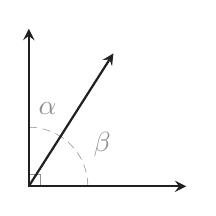
\begin{tikzpicture}
                        \draw[help lines] (0,0.15) -| (0.15,0);
                        \draw[help lines, densely dashed] (0.75,0) arc[start angle=0, end angle=57.5, radius=0.75] node[right, shift={(0.3,-0.1)}] {$\beta$};
                        \draw[help lines, densely dashed] (0,0.75) arc[start angle=90, end angle=57.5, radius=0.75] node[right, shift={(-0.4,0.35)}] {$\alpha$};
                        \draw[black, thick, {stealth}-{stealth}] (0,2) |- (2,0);
                        \draw[black, thick, -{stealth}] (0,0) -- (57.5:2);
                    \end{tikzpicture}
                \end{SummaryExtensionBox}
                
                \begin{SummaryExtensionBox}[title=Supplementary angles, sidebyside, righthand ratio=0.45, leftlower=0pt, rightlower=0pt, center lower]
                    \begin{itemize}[leftmargin=*]
                        \item In this case, the angles $\alpha$ and $\beta$ are complimentary, as $\alpha + \beta = 180^{\circ}$.
                    \end{itemize}
                    \tcblower
                    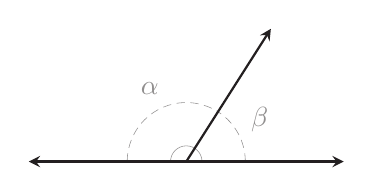
\begin{tikzpicture}
                        \draw[help lines] (0.2,0) arc[start angle=0, end angle=180, radius=0.2];
                        \draw[help lines, densely dashed] (0.75,0) arc[start angle=0, end angle=57.5, radius=0.75] node[right, shift={(0.3,-0.1)}] {$\beta$};
                        \draw[help lines, densely dashed] (-0.75,0) arc[start angle=180, end angle=57.5, radius=0.75] node[right, shift={(-1.1,0.3)}] {$\alpha$};
                        \draw[black, thick, {stealth}-{stealth}] (-2,0) -- (2,0);
                        \draw[black, thick, -{stealth}] (0,0) -- (57.5:2);
                    \end{tikzpicture}
                \end{SummaryExtensionBox}
            \end{SummaryBox}
            
            \begin{SummaryBox}[title=Angles formed by intersecting lines, breakable]
                \begin{SummaryExtensionBox}[title=Vertically opposite angles, sidebyside, righthand ratio=0.45, leftlower=0pt, rightlower=0pt, center lower]
                    \begin{itemize}[leftmargin=*]
                        \item In this case, $\angle AXC = \angle DXB$ and $\angle DXA = \angle BXC$.
                    \end{itemize}
                    \tcblower
                    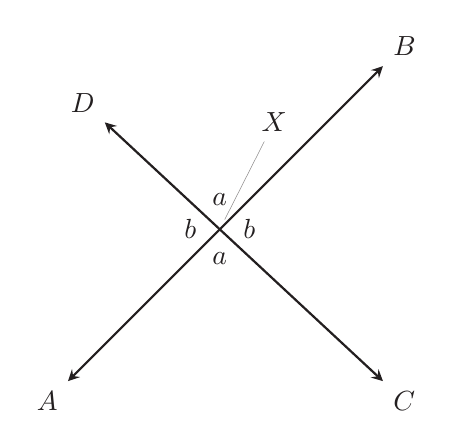
\begin{tikzpicture}
                        \draw[black, thick, name path=p1, {stealth}-{stealth}] (-2,-2) node[below left] {$A$} -- (2,2) node[above right] {$B$};
                        \draw[black, thick, name path=p2, {stealth}-{stealth}] (2,-2) node[below right] {$C$} -- (140:2) node[above left] {$D$};
                        \path[name intersections={of=p1 and p2, by={X}}];
                        \node[black, above, yshift=5] at (X) {$a$};
                        \node[black, below, yshift=-5] at (X) {$a$};
                        \node[black, left, xshift=-5] at (X) {$b$};
                        \node[black, right, xshift=5] at (X) {$b$};
                        \node[pin={[pin distance=30]70:$X$}] at (X) {};
                    \end{tikzpicture}
                \end{SummaryExtensionBox}
                
                \begin{SummaryExtensionBox}[title=Angles formed by a transversal, sidebyside, righthand ratio=0.45, leftlower=0pt, rightlower=0pt, center lower]
                    \begin{itemize}
                        \item A \textbf{transversal} is a line which crosses two or more lines.
                        \item In this case, the lines $AB$ and $CD$ are \textbf{parallel}, which is denoted by $AB \parallel CD$.
                        \item \textbf{Vertically opposite angles}:
                        \begin{itemize}[topsep=0pt]
                            \item $\angle CYF = \angle XYD$
                            \item $\angle YFD = \angle CYX$
                            \item $\angle AXY = \angle EXB$
                            \item $\angle AXE = \angle YXB$
                        \end{itemize}
                        \item \textbf{Alternate interior angles}:
                        \begin{itemize}
                            \item $\angle AXY = \angle DYX$
                            \item $\angle CYX = \angle BXY$
                        \end{itemize}
                        \item \textbf{Alternate exterior angles}:
                        \begin{itemize}
                            \item $\angle FYD = \angle AXE$
                            \item $\angle FYC = \angle EXB$
                        \end{itemize}
                        \item \textbf{Corresponding angles}:
                        \begin{itemize}
                            \item $\angle FYD = \angle YXB$
                            \item $\angle FYC = \angle YXA$
                            \item $\angle EXB = \angle XYD$
                            \item $\angle EXA = \angle XYC$
                        \end{itemize}
                        \item \textbf{Same side interior angles (supplementary)}:
                        \begin{itemize}
                            \item $\angle XYD + \angle YXB = 180^{\circ}$
                            \item $\angle AXY + \angle CYX = 180^{\circ}$
                        \end{itemize}
                    \end{itemize}
                    \tcblower
                    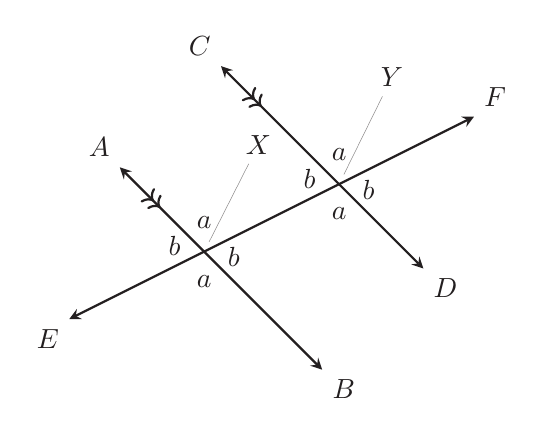
\begin{tikzpicture}[scale=0.6425]
                        \draw[black, thick, name path=p1, {stealth}-{stealth}, ->>-] (-2,2) node[above left] {$A$} -- (2,-2) node[below right] {$B$};
                        \draw[black, thick, name path=p2, {stealth}-{stealth}, ->>-] (0,4) node[above left] {$C$} -- (4,0) node[below right] {$D$};
                        \draw[black, thick, name path=t1, {stealth}-{stealth}] (-3,-1) node[below left] {$E$} -- (5,3) node[above right] {$F$};
                        \path[name intersections={of=t1 and p1, by={X}}];
                        \path[name intersections={of=t1 and p2, by={Y}}];
                        \node[black, above, yshift=5] at (Y) {$a$};
                        \node[black, below, yshift=-5] at (Y) {$a$};
                        \node[black, right, xshift=5, yshift=-2] at (Y) {$b$};
                        \node[black, left, xshift=-5, yshift=2] at (Y) {$b$};
                        \node[black, above, yshift=5] at (X) {$a$};
                        \node[black, below, yshift=-5] at (X) {$a$};
                        \node[black, right, xshift=5, yshift=-2] at (X) {$b$};
                        \node[black, left, xshift=-5, yshift=2] at (X) {$b$};
                        \node[pin={[pin distance=30]70:$X$}] at (X) {};
                        \node[pin={[pin distance=30]70:$Y$}] at (Y) {};
                    \end{tikzpicture}
                \end{SummaryExtensionBox}
            \end{SummaryBox}

        \pagebreak
        
        \section{Pseudocode}
            
            \begin{SummaryBox}[title=What is pseudocode]
                We can use computers to perform calculations using algorithms (\textit{e.g.,} Newton's method, the bisection method, etc.). To accomplish this, we need to describe to the computer how to carry out a specific algorithm. We use \textbf{pseudocode} to do this. A computer would need to have the algorithm described using a programming language, but pseudocode provides a language-agnostic way to accomplish the same thing using an informal set of tokens and keywords.
            \end{SummaryBox}

            \begin{SummaryBox}[title=Concepts of pseudocode, breakable]
                \begin{SummaryExtensionBox}[title=Comments]
                    Comments are lines ignored by the program. They are meant to serve as explanatory sentences or anything else that the reader/programmer should know, but isn't necessarily an instruction for the program.
                    \begin{codebox}{Comments}
                        # This is a comment and it will be ignored.
                        |\( \textit{instructions}\dots \)|
                        # It is here only for the reader/programmer.
                        |\( \textit{more instructions}\dots \)|
                    \end{codebox}
                \end{SummaryExtensionBox}
                
                \begin{SummaryExtensionBox}[title=Conditional statements]
                    Oftentimes, our programs need to make decisions influenced by other things. We can use \inlinemintvcaa{If} and \inlinemintvcaa{Else} statements.
                    \begin{codebox}{Conditional statements}
                        If |\( \textit{condition} \)| Then
                            |\( \textit{follow these instructions} \)|
                        Else If |\( \textit{second condition} \)| Then
                            |\( \textit{if the first condition was false, follow these instructions instead} \)|
                        Else
                            |\( \textit{if all else fails, try this instead} \)|
                    \end{codebox}
                \end{SummaryExtensionBox}
                
                \begin{SummaryExtensionBox}[title=For loops]
                    When we want to repeat something in a finite sequence of steps, we can use a \inlinemintvcaa{For} loop.
                    \begin{codeboxwithcomment}{For loop}[0.25\linewidth]{In a \inlinemintvcaa{For} loop, \( \textit{starting\_index} \leq n \).\vspace{0.65\baselineskip}\\If \( \textit{starting\_index} = n \), then the \inlinemintvcaa{For} loop won't execute.}
                        For |\( \textit{variable\_name} \)| From |\( \textit{starting\_index} \)| To |\( n \)|
                            |\( \textit{execute these lines } (n - \textit{starting\textunderscore{}index}) \textit{ times} \)|
                        EndFor
                    \end{codeboxwithcomment}
                \end{SummaryExtensionBox}
                
                \begin{SummaryExtensionBox}[title=While loops]
                    When we want to repeat something an infinite amount of time or when we don't know the number of iterations required to complete a task, a \inlinemintvcaa{While} loop can be used.
                    \begin{codeboxwithcomment}{While loop}[0.5\linewidth]{At the end of every iteration, a \inlinemintvcaa{While} loop goes back to the start, and checks if \textit{condition} is still \inlinemintvcaa{True}.\vspace{0.65\baselineskip}\\If \textit{condition} is \inlinemintvcaa{False} to begin with, then the \inlinemintvcaa{While} loop will never run.}
                        While |\( \textit{condition} \)| Do
                            |\( \textit{execute these instructions} \)|
                        EndWhile
                    \end{codeboxwithcomment}
                \end{SummaryExtensionBox}
                
                \begin{SummaryExtensionBox}[title=Functions]
                    Functions provide a way of isolating code for readability and repetition. A \inlinemintvcaa{Function} takes zero, one, or more arguments and returns a value. A function has to be \textbf{defined}, and later \textbf{called} to be executed.
                    \begin{codeboxwithcomment}{Functions}{Leave the \inlinemintvcaa{Function}'s arguments blank if it takes no arguments.\vspace{0.65\baselineskip}\\Finally, calling the function is required to execute the code within it.}
                        Define |\( \textit{function\_name} \)|(|\( \textit{arg\_1} \)|, |\( \textit{arg\_2} \)|, |\( \dots \)|)
                            |\( \textit{execute these instructions} \)|
                            Return |\( \textit{output\_value} \)|
                        
                        |\( \textit{function\_name} \)|(|\( \textit{arg\_1} \)|, |\( \textit{arg\_2} \)|, |\( \dots \)|)
                    \end{codeboxwithcomment}
                \end{SummaryExtensionBox}
                
                \begin{SummaryExtensionBox}[title=Variables]
                    Variables, much like in pure math, can be used to store things. Just like we can say \( x = \frac{-b \pm \sqrt{b^2 - 4ac}}{2a} \) in math, we can say the same in pseudocode with one caveat: in this specific case, \( x \) has two values (owing to the use of the \( \pm \) symbol), but in pseudocode, a variable can only have one value at a time. So, to get both our values, we would need to make two variables (one for \( +\sqrt{\Delta} \) and one for \( -\sqrt{\Delta} \)).
                    \begin{codeboxwithcomment}{Variables}[0.4\linewidth]{In pseudocode, variables \textit{store} values, so we typically see the use of \( \leftarrow \) instead of the \( = \) sign.}
                        |\( a \)| |\( \leftarrow \)| 42
                        |\( b \)| |\( \leftarrow \)| |\( a \)| - 43
                    \end{codeboxwithcomment}
                \end{SummaryExtensionBox}

                \begin{SummaryExtensionBox}[title=All concepts used in conjunction]
                    \begin{codebox}{Sum of the factorial of the first \( \bm{n} \) natural numbers}
                        Define factorial(x)
                            # Returns x$!$. This function will not work for negative integers; designed only for x${} \in \mathbb{N} \cup \curls{0}$.
                            result |\( \leftarrow \)| 1  # multiplication happens, so result${} \neq 0$
                            i |\( \leftarrow \)| x
                            While i > 0 Do
                                result |\( \leftarrow \)| result * i  # new $\text{``}$result$\text{''}$ = old $\text{``}$result$\text{''} \times \text{``}$i$\text{''}$
                                i |\( \leftarrow \)| i - 1  # Decrement i with each iteration
                            EndWhile
                            Return result
                        
                        Define factorial_sum(n)
                            # Returns the sum of the factorials of every natural number up to n (inclusive upper bound).
                            If n |\( \leq \)| 0 Then
                                Return -1  # Invalid input of $\text{``}$n$\text{''}$
                            
                            result |\( \leftarrow \)| 0  # $\text{``}$result$\text{''}$ is different the variable in the factorial function.
                            For i From 1 To (n + 1)  # $\text{``}$i$\text{''}$ is different too
                                result |\( \leftarrow \)| result + factorial(i)
                            EndFor
    
                            Return result
                        
                        factorial_sum(10)  # Gets the sum of the factorials of 1, 2, ..., 10.
                    \end{codebox}
                \end{SummaryExtensionBox}
            \end{SummaryBox}
            
        \begin{landscape}
            
            \section{Counting methods}

                \begin{SummaryBox}[title=Pascal's triangle, leftlower=0pt, rightlower=0pt]
                    \begin{itemize}
                        \item Featured below is \textbf{pascal's triangle}, in which each row $n$ and column $k$ correspond to $\binom{n}{k}$.
                        \begin{itemize}
                            \item Binomial expansion: $(a+b)^n = \sum\limits_{k=0}^n \binom{n}{k} \cdot a^{n-k} \cdot b^k \quad\quad \text{and} \quad\quad (qa+b)^n = \sum\limits_{k=0}^n \binom{n}{k} \cdot (q \cdot a)^{n-k} \cdot b^k$
                        \end{itemize}
                    \end{itemize}
                    \tcblower
                    \vspace{-2\belowdisplayskip}
                    \vspace{2mm}
                    \begin{table}[H]
                        \centering
                        \begin{tblr}{%
                                        colspec={Q[r,mode=dmath]|*{16}{Q[r,mode=math]}},
                                        cell{1}{1}={r=1,c=17}{l},
                                    }
                            n   &   &       &       &       &       &       &       &       &           &           &           &           &           &       &       &       \\
                            \cline{1}
                            0   & 1 &       &       &       &       &       &       &       &           &           &           &           &           &       &       &       \\
                            1   & 1 & 1     &       &       &       &       &       &       &           &           &           &           &           &       &       &       \\
                            2   & 1 & 2     & 1     &       &       &       &       &       &           &           &           &           &           &       &       &       \\
                            3   & 1 & 3     & 3     & 1     &       &       &       &       &           &           &           &           &           &       &       &       \\
                            4   & 1 & 4     & 6     & 4     & 1     &       &       &       &           &           &           &           &           &       &       &       \\
                            5   & 1 & 5     & 10    & 10    & 5     & 1     &       &       &           &           &           &           &           &       &       &       \\
                            6   & 1 & 6     & 15    & 20    & 15    & 6     & 1     &       &           &           &           &           &           &       &       &       \\
                            7   & 1 & 7     & 21    & 35    & 35    & 21    & 7     & 1     &           &           &           &           &           &       &       &       \\
                            8   & 1 & 8     & 28    & 56    & 70    & 56    & 28    & 8     & 1         &           &           &           &           &       &       &       \\
                            9   & 1 & 9     & 36    & 84    & 126   & 126   & 84    & 36    & 9         & 1         &           &           &           &       &       &       \\
                            10  & 1 & 10    & 45    & 120   & 210   & 252   & 210   & 120   & 45        & 10        & 1         &           &           &       &       &       \\
                            11  & 1 & 11    & 55    & 165   & 330   & 462   & 462   & 330   & 165       & 55        & 11        & 1         &           &       &       &       \\
                            12  & 1 & 12    & 66    & 220   & 495   & 792   & 924   & 792   & 495       & 220       & 66        & 12        & 1         &       &       &       \\
                            13  & 1 & 13    & 78    & 286   & 715   & 1287  & 1716  & 1716  & 1287      & 715       & 286       & 78        & 13        & 1     &       &       \\
                            14  & 1 & 14    & 91    & 364   & 1001  & 2002  & 3003  & 3432  & 3003      & 2002      & 1001      & 364       & 91        & 14    & 1     &       \\
                            15  & 1 & 15    & 105   & 455   & 1365  & 3003  & 5005  & 6435  & 6435      & 5005      & 3003      & 1365      & 455       & 105   & 15    & 1     \\
                            \hline
                            k   & 0 & 1     & 2     & 3     & 4     & 5     & 6     & 7     & 8         & 9         & 10        & 11        & 12        & 13    & 14    & 15    \\
                            \hline
                        \end{tblr}
                    \end{table}
                \end{SummaryBox}
                
            
        \pagebreak
        
        \section{Base functions}
            
            \tikzset{%
                baseline=(current bounding box).north
            }
            
            \pgfplotsset{ trig format plots=rad }
            
            \begin{longtblr}[caption={Base graphs}, label={tblr:basegraphs}]{hlines, colspec={| X[c,0.1] | X[c,0.15] | X[c,0.05] | X[c,0.05] | X[c,0.3] | X[c,0.1] | X[c,0.15] |}, row{1}={font=\bfseries, m, bg=Apricot!50}, row{2-Z}={ht=5cm}, rowhead=1}
                Rule                                & Implied domain                            & Range                             & Parity    & Graph                                                             & Inverse                           & Asymptote \\
                $x^n, n\text{ is even}$             & $\mathbb{R}$                              & $[0,\infty)$                      & Even      & {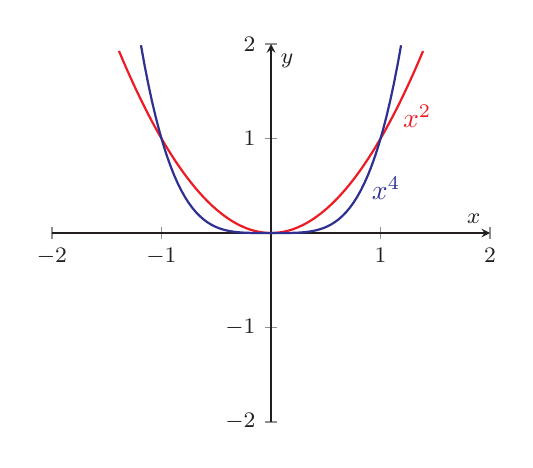
\begin{tikzpicture}
                                                                                                                                                      \begin{axis}[
                                                                                                                                                          My Style 2,
                                                                                                                                                          xmin=-2,
                                                                                                                                                          xmax=2,
                                                                                                                                                          ymin=-2,
                                                                                                                                                          ymax=2
                                                                                                                                                      ]
                                                                                                                                                          \addplot[red,thick] {x^2} node[pos=0.85, right] {$x^2$};
                                                                                                                                                          \addplot[blue,thick] {x^4} node[pos=0.7, right] {$x^4$};
                                                                                                                                                      \end{axis}
                                                                                                                                                  \end{tikzpicture}}                                                & $\sqrt[n]{x}, n\text{ is even}$   & None \\
                $x^n, n\text{ is odd}$              & $\mathbb{R}$                              & $\mathbb{R}$                      & Odd       & {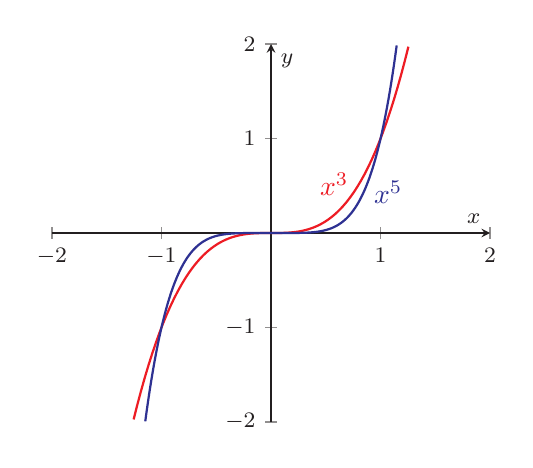
\begin{tikzpicture}
                                                                                                                                                      \begin{axis}[
                                                                                                                                                          My Style 2,
                                                                                                                                                          xmin=-2,
                                                                                                                                                          xmax=2,
                                                                                                                                                          ymin=-2,
                                                                                                                                                          ymax=2
                                                                                                                                                      ]
                                                                                                                                                          \addplot[red,thick] {x^3} node[pos=0.7, left] {$x^3$};
                                                                                                                                                          \addplot[blue,thick, samples=5003] {x^5} node[pos=0.7, right] {$x^5$};
                                                                                                                                                      \end{axis}
                                                                                                                                                  \end{tikzpicture}}                                                & $\sqrt[n]{x}, n\text{ is odd}$    & None \\
                $\frac{1}{x}$                       & $\mathbb{R} \setminus \curls*{0}$         & $\mathbb{R}$                      & Odd       & {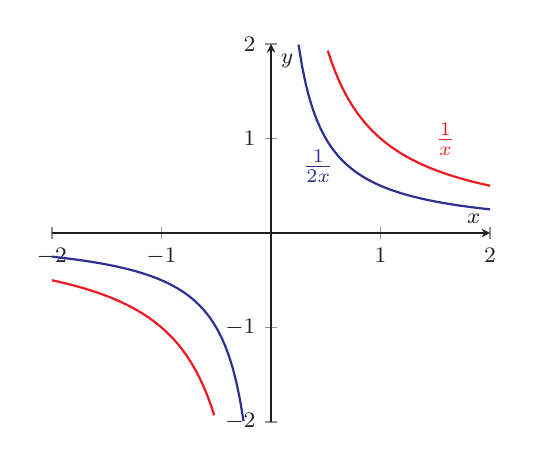
\begin{tikzpicture}
                                                                                                                                                      \begin{axis}[
                                                                                                                                                          My Style 2,
                                                                                                                                                          xmin=-2,
                                                                                                                                                          xmax=2,
                                                                                                                                                          ymin=-2,
                                                                                                                                                          ymax=2
                                                                                                                                                      ]
                                                                                                                                                          \addplot[red,thick] {1/x} node[pos=0.65, above right] {$\frac{1}{x}$};
                                                                                                                                                          \addplot[blue,thick] {1/(2*x)} node[pos=0.6, below left, shift={(axis direction cs:0.1,0.1)}] {$\frac{1}{2x}$};
                                                                                                                                                      \end{axis}
                                                                                                                                                  \end{tikzpicture}}                                                & $\frac{1}{x}$                     & {$y=0$\\$x=0$} \\
                $\frac{1}{x^n}, n\text{ is even}$   & $\mathbb{R} \setminus \curls*{0}$         & $\mathbb{R}^+$                    & Even      & {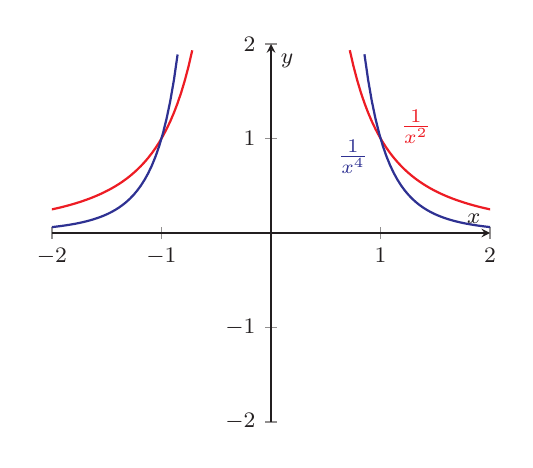
\begin{tikzpicture}
                                                                                                                                                      \begin{axis}[
                                                                                                                                                          My Style 2,
                                                                                                                                                          xmin=-2,
                                                                                                                                                          xmax=2,
                                                                                                                                                          ymin=-2,
                                                                                                                                                          ymax=2
                                                                                                                                                      ]
                                                                                                                                                          \addplot[red,thick] {1/(x^2)} node[pos=0.61, above right] {$\frac{1}{x^2}$};
                                                                                                                                                          \addplot[blue,thick] {1/(x^4)} node[pos=0.575, below left] {$\frac{1}{x^4}$};
                                                                                                                                                      \end{axis}
                                                                                                                                                  \end{tikzpicture}}                                                & $\pm\frac{1}{\sqrt[n]{x}}$        & {$y=0$\\$x=0$} \\
                $\frac{1}{x^n}, n\text{ is odd}$    & $\mathbb{R} \setminus \curls*{0}$         & $\mathbb{R} \setminus \curls*{0}$ & Odd       & {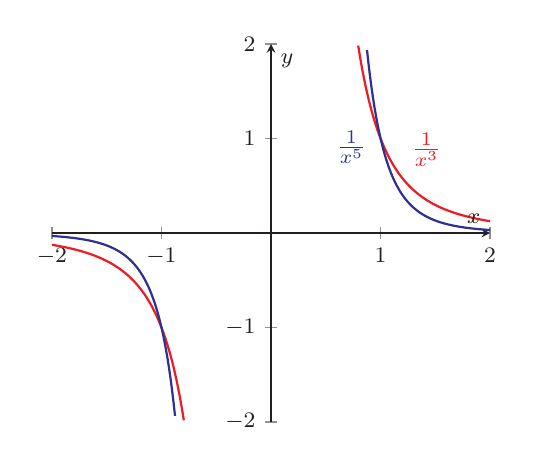
\begin{tikzpicture}
                                                                                                                                                      \begin{axis}[
                                                                                                                                                          My Style 2,
                                                                                                                                                          xmin=-2,
                                                                                                                                                          xmax=2,
                                                                                                                                                          ymin=-2,
                                                                                                                                                          ymax=2
                                                                                                                                                      ]
                                                                                                                                                          \addplot[red,thick,domain=-2:2] {1/(x^3)} node[pos=0.8, above right] {$\frac{1}{x^3}$};
                                                                                                                                                          \addplot[blue,thick,domain=-2:2] {1/(x^5)} node[pos=0.65, below left] {$\frac{1}{x^5}$};
                                                                                                                                                      \end{axis}
                                                                                                                                                  \end{tikzpicture}}                                                & $\frac{1}{\sqrt[n]{x}}$           & {$y=0$\\$x=0$} \\
                $a^x, {0<a<1}$                      & $\mathbb{R}$                              & $\mathbb{R}^+$                    & None      & {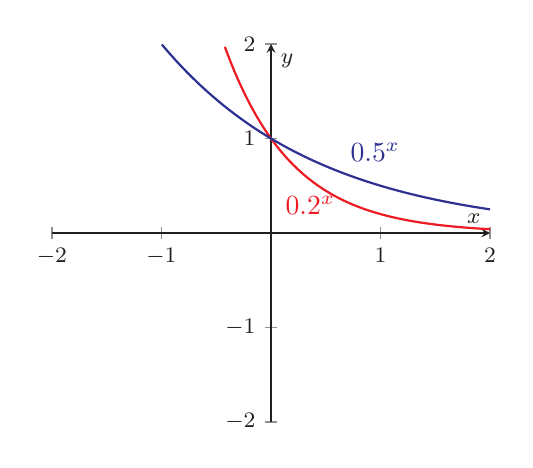
\begin{tikzpicture}
                                                                                                                                                      \begin{axis}[
                                                                                                                                                          My Style 2,
                                                                                                                                                          xmin=-2,
                                                                                                                                                          xmax=2,
                                                                                                                                                          ymin=-2,
                                                                                                                                                          ymax=2
                                                                                                                                                      ]
                                                                                                                                                          \addplot[red,thick,domain=-2:2] {(0.2)^x} node[pos=0.5625, below left, shift={(axis direction cs:0.1,0.1)}] {$0.2^x$};
                                                                                                                                                          \addplot[blue,thick,domain=-2:2] {(0.5)^x} node[pos=0.6, above right] {$0.5^x$};
                                                                                                                                                      \end{axis}
                                                                                                                                                  \end{tikzpicture}}                                                & $\sqrt[a]{x}$                     & $y=0$ \\
                $a^x, a>1$                          & $\mathbb{R}$                              & $\mathbb{R}^+$                    & None      & {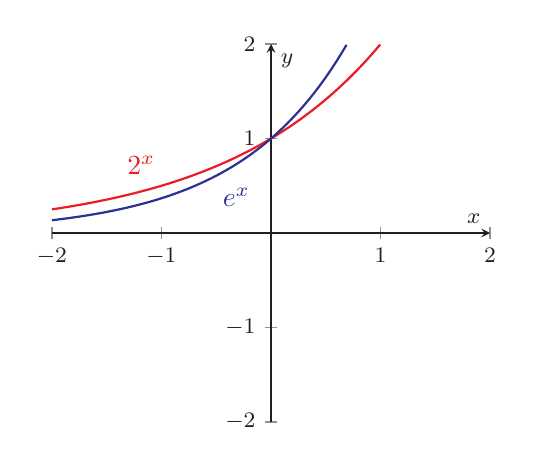
\begin{tikzpicture}
                                                                                                                                                      \begin{axis}[
                                                                                                                                                          My Style 2,
                                                                                                                                                          xmin=-2,
                                                                                                                                                          xmax=2,
                                                                                                                                                          ymin=-2,
                                                                                                                                                          ymax=2
                                                                                                                                                      ]
                                                                                                                                                          \addplot[red,thick,domain=-2:2] {2^x} node[pos=0.3, above left] {$2^x$};
                                                                                                                                                          \addplot[blue,thick,domain=-2:2] {exp(x)} node[pos=0.45, below right] {$e^x$};
                                                                                                                                                      \end{axis}
                                                                                                                                                  \end{tikzpicture}}                                                & $\sqrt[a]{x}$                     & $y=0$ \\
                $\sin(x)$                           & $\mathbb{R}$                              & $[-1,1]$                          & Odd       & {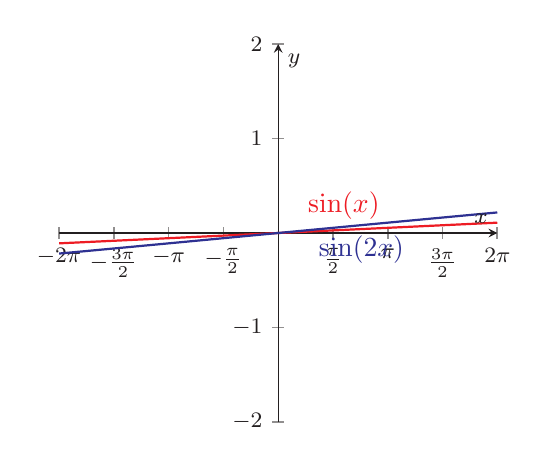
\begin{tikzpicture}
                                                                                                                                                      \begin{axis}[
                                                                                                                                                          My Style 2,
                                                                                                                                                          xmin=-2*pi,
                                                                                                                                                          xmax=2*pi,
                                                                                                                                                          ymin=-2,
                                                                                                                                                          ymax=2,
                                                                                                                                                          xtick={-2*pi,-(3*pi)/2,-pi,-pi/2,pi/2,pi,(3*pi)/2,2*pi},
                                                                                                                                                          xticklabels={$-2\pi$,$-\frac{3\pi}{2}$,$-\pi$,$-\frac{\pi}{2}$,$\frac{\pi}{2}$,$\pi$,$\frac{3\pi}{2}$,$2\pi$}
                                                                                                                                                      ]
                                                                                                                                                          \addplot[red,thick,domain=-2*pi:2*pi] {sin(x)} node[pos=0.65, above] {$\sin(x)$};
                                                                                                                                                          \addplot[blue,thick,domain=-2*pi:2*pi] {sin(2*x)} node[pos=0.69, below] {$\sin(2x)$};
                                                                                                                                                      \end{axis}
                                                                                                                                                  \end{tikzpicture}}                                                & $\sin^{-1}(x)$                    & None  \\
                $\cos(x)$                           & $\mathbb{R}$                              & $[-1,1]$                          & Even      & {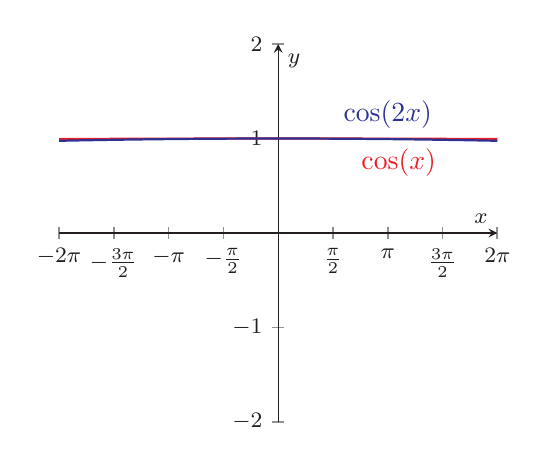
\begin{tikzpicture}
                                                                                                                                                      \begin{axis}[
                                                                                                                                                          My Style 2,
                                                                                                                                                          xmin=-2*pi,
                                                                                                                                                          xmax=2*pi,
                                                                                                                                                          ymin=-2,
                                                                                                                                                          ymax=2,
                                                                                                                                                          xtick={-2*pi,-(3*pi)/2,-pi,-pi/2,pi/2,pi,(3*pi)/2,2*pi},
                                                                                                                                                          xticklabels={$-2\pi$,$-\frac{3\pi}{2}$,$-\pi$,$-\frac{\pi}{2}$,$\frac{\pi}{2}$,$\pi$,$\frac{3\pi}{2}$,$2\pi$}
                                                                                                                                                      ]
                                                                                                                                                          \addplot[red,thick,domain=-2*pi:2*pi] {cos(x)} node[pos=0.775, below] {$\cos(x)$};
                                                                                                                                                          \addplot[blue,thick,domain=-2*pi:2*pi] {cos(2*x)} node[pos=0.75, above] {$\cos(2x)$};
                                                                                                                                                      \end{axis}
                                                                                                                                                  \end{tikzpicture}}                                                & $\cos^{-1}(x)$                    & None  \\
                $\tan(x)$                           & $x\neq\frac{(2n-1)\pi}{2},n\in\mathbb{Z}$ & $\mathbb{R}$                      & Odd       & {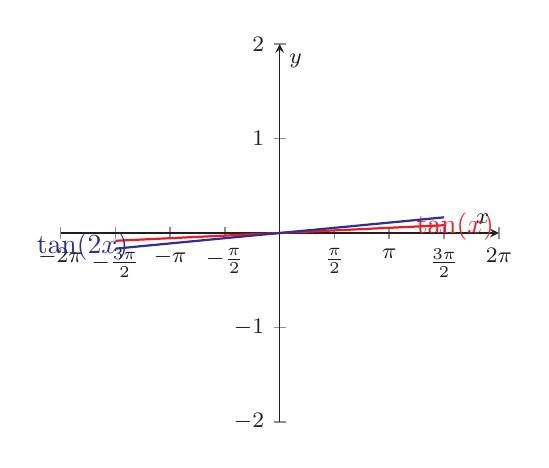
\begin{tikzpicture}
                                                                                                                                                      \begin{axis}[
                                                                                                                                                          My Style 2,
                                                                                                                                                          xmin=-2*pi,
                                                                                                                                                          xmax=2*pi,
                                                                                                                                                          ymin=-2,
                                                                                                                                                          ymax=2,
                                                                                                                                                          clip=false,
                                                                                                                                                          xtick={-2*pi,-(3*pi)/2,-pi,-pi/2,pi/2,pi,(3*pi)/2,2*pi},
                                                                                                                                                          xticklabels={$-2\pi$,$-\frac{3\pi}{2}$,$-\pi$,$-\frac{\pi}{2}$,$\frac{\pi}{2}$,$\pi$,$\frac{3\pi}{2}$,$2\pi$}
                                                                                                                                                      ]
                                                                                                                                                          \addplot[red,thick,domain=-(3*pi)/2:(3*pi)/2] {tan(x)} node[pos=0.885, right] {$\tan(x)$};
                                                                                                                                                          \addplot[blue,thick,domain=-(3*pi)/2:(3*pi)/2,samples=800] {tan(2*x)} node[pos=0.07, left, shift={(axis direction cs:0,0)}] {$\tan(2x)$};
                                                                                                                                                      \end{axis}
                                                                                                                                                  \end{tikzpicture}}                                                & $\tan^{-1}(x)$                    & $x=\frac{(2n-1)\pi}{2}$ \\
                $\log_a(x)$, $0<a<1$                & $\mathbb{R}^+$                            & $\mathbb{R}$                      & None      & {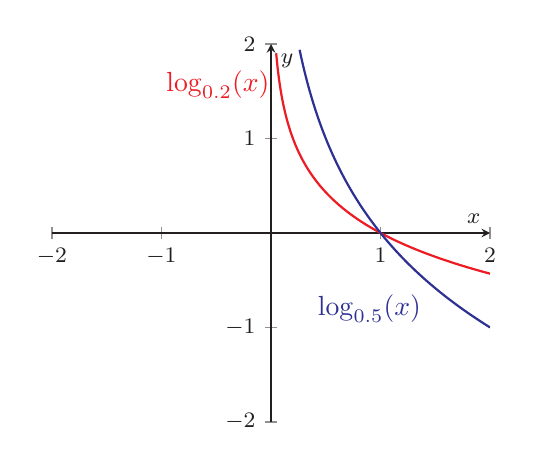
\begin{tikzpicture}
                                                                                                                                                      \begin{axis}[
                                                                                                                                                          My Style 2,
                                                                                                                                                          xmin=-2,
                                                                                                                                                          xmax=2,
                                                                                                                                                          ymin=-2,
                                                                                                                                                          ymax=2
                                                                                                                                                      ]
                                                                                                                                                          \addplot[red,thick,domain=-2:2] {(ln(x))/(ln(0.2))} node[pos=0.1, left] {$\log_{0.2}(x)$};
                                                                                                                                                          \addplot[blue,thick,domain=-2:2] {(ln(x))/(ln(0.5))} node[pos=0.8, below left] {$\log_{0.5}(x)$};
                                                                                                                                                      \end{axis}
                                                                                                                                                  \end{tikzpicture}}                                                & $a^x, 0<a<1$                      & $y=0$ \\
                $\log_a(x), a>1$                    & $\mathbb{R}^+$                            & $\mathbb{R}$                      & None      & {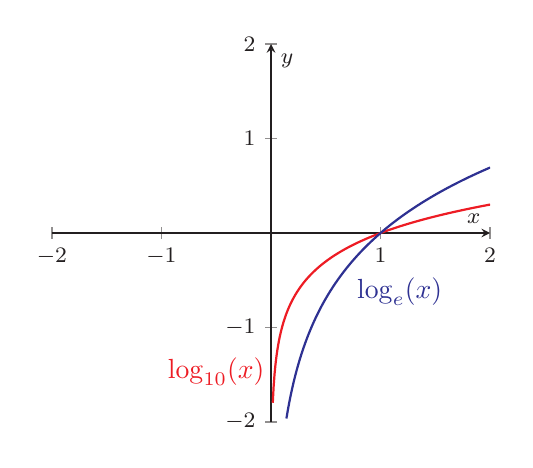
\begin{tikzpicture}
                                                                                                                                                      \begin{axis}[
                                                                                                                                                          My Style 2,
                                                                                                                                                          xmin=-2,
                                                                                                                                                          xmax=2,
                                                                                                                                                          ymin=-2,
                                                                                                                                                          ymax=2
                                                                                                                                                      ]
                                                                                                                                                          \addplot[red,thick,domain=-2:2,samples=501] {((ln(x))/(ln(10)))} node[pos=0.1, left, shift={(axis direction cs:0,0)}] {$\log_{10}(x)$};
                                                                                                                                                          \addplot[blue,thick,domain=-2:2] {ln(x)} node[pos=0.5, below right] {$\log_e(x)$};
                                                                                                                                                      \end{axis}
                                                                                                                                                  \end{tikzpicture}}                                                & $a^x, a>1$                        & $y=0$ \\
                $\sqrt[n]{x}, n\text{ is even}$     & $\mathbb{R}^+ \cup \curls*{0}$            & $\mathbb{R}^+$                    & None      & {\begin{tikzpicture}
                                                                                                                                                      \begin{axis}[
                                                                                                                                                          My Style 2,
                                                                                                                                                          xmin=-2,
                                                                                                                                                          xmax=2,
                                                                                                                                                          ymin=-2,
                                                                                                                                                          ymax=2
                                                                                                                                                      ]
                                                                                                                                                          \addplot[red,thick,domain=-2:2,samples=1001] {x^(1/2)} node[pos=0.8, above left] {$\sqrt{x}$};
                                                                                                                                                          \addplot[blue,thick,domain=-2:2,samples=1001] {x^(1/4)} node[pos=0.6, below right] {$\sqrt[4]{x}$};
                                                                                                                                                      \end{axis}
                                                                                                                                                  \end{tikzpicture}}                                                & $x^n$                             & None \\
                $\sqrt[n]{x}, n\text{ is odd}$      & $\mathbb{R}$                              & $\mathbb{R}$                      & None      & {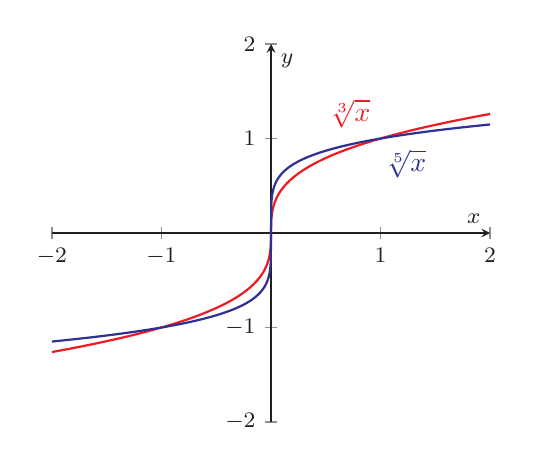
\begin{tikzpicture}
                                                                                                                                                      \begin{axis}[
                                                                                                                                                          My Style 2,
                                                                                                                                                          xmin=-2,
                                                                                                                                                          xmax=2,
                                                                                                                                                          ymin=-2,
                                                                                                                                                          ymax=2
                                                                                                                                                      ]
                                                                                                                                                          \addplot[red,thick,domain=0:2,samples=1001] {x^(1/3)} node[pos=0.6, above left] {$\sqrt[3]{x}$};
                                                                                                                                                          \addplot[red,thick,domain=-2:0,samples=1001] {-((-x)^(1/3))};
                                                                                                                                                          \addplot[blue,thick,domain=0:2,samples=1001] {x^(1/5)} node[pos=0.6, below right] {$\sqrt[5]{x}$};
                                                                                                                                                          \addplot[blue,thick,domain=-2:0,samples=1001] {-((-x)^(1/5))};
                                                                                                                                                      \end{axis}
                                                                                                                                                  \end{tikzpicture}}                                                & $x^n$                             & None \\
                
            \end{longtblr}
            
        \end{landscape}
        
    
\end{document}